%%%%%%%%%%%%%%%%%%%%%%%%%%%%%%%%%%%%%%%%%%%%%%%%%%%%%%%%%%%%%%%%%%%%%%%%%%%%%%%%%%%%%%
%% Author:      Nils Weber and Maximilian Stiefel
%% Date:        23.12.2017
%% University:  Uppsala Universitet
%% Department:  Institutionen för informationsteknologi 
%% Course:      Embedded Control System Project
%% Project:     PRECISELY CONTROLLED DIY ETCHING MACHINE 
%%				FOR USAGE AT HOME AND IN SMALL LABS
%%%%%%%%%%%%%%%%%%%%%%%%%%%%%%%%%%%%%%%%%%%%%%%%%%%%%%%%%%%%%%%%%%%%%%%%%%%%%%%%%%%%%%

\documentclass{report}

%%%%%%%%%%%%%%%%%%%%%%%%%%%%%%%%%%%%%%%%%%%%%%%%%%%%%%%%%%%%%%%%%%%%%%%%%%%%%%%%%%%%%%
% Preamble
%%%%%%%%%%%%%%%%%%%%%%%%%%%%%%%%%%%%%%%%%%%%%%%%%%%%%%%%%%%%%%%%%%%%%%%%%%%%%%%%%%%%%%

% Encoding of the input
\usepackage[utf8]{inputenc}

% Geometry stuff
\usepackage[head=24pt,a4paper,lmargin={2.5cm},rmargin={2.5cm},tmargin={2.5cm},
bmargin={2.5cm}]{geometry}

% For graphics
\usepackage{graphicx}
\usepackage{float}

% For code highlighting
\usepackage{minted}

% For shaded
\usepackage{xcolor}
\usepackage{framed}
\definecolor{shadecolor}{gray}{0.9}

% For some symbols
\usepackage{textcomp}
%\usepackage{eurosans}

% For math
\usepackage{amssymb}
\usepackage{amsmath}

\setlength{\parindent}{0em} 

% For title formatting 
\usepackage{titlesec} 

\titleformat%
{\chapter}%
[block]%
{\bfseries\Huge}%
{\thechapter\hspace{1cm}}%
{0pt}%
{\bfseries\Huge}%

% For SI units.
\usepackage{siunitx}

% Input definition macros
%%%%%%%%%%%%%%%%%%%%%%%%%%%%%%%%%%%%%%%%%%%%%%%%%%%%%%%%%%%%%%%%%%%%%%%%%%%%%%%%%%%%%%
%% Author:      Nils Weber and Maximilian Stiefel
%% Date:        23.12.2017
%% University:  Uppsala Universitet
%% Department:  Institutionen för informationsteknologi 
%% Course:      Embedded Control System Project
%% Project:     PRECISELY CONTROLLED DIY ETCHING MACHINE 
%%				FOR USAGE AT HOME AND IN SMALL LABS
%%%%%%%%%%%%%%%%%%%%%%%%%%%%%%%%%%%%%%%%%%%%%%%%%%%%%%%%%%%%%%%%%%%%%%%%%%%%%%%%%%%%%%

\newcommand{\mytitle}{\uppercase{Precisely Controlled DIY Etching Machine For Usage at Home and in Small Labs}}
\newcommand{\mytypeofwork}{Project Report}
\newcommand{\mycourse}{Embedded Control Systems} 
\newcommand{\myuniversity}{Uppsala University}
\newcommand{\mydepartement}{Information Technology}
\newcommand{\myauthora}{Nils Weber}
\newcommand{\myauthorb}{Maximilian Stiefel}
\newcommand{\myauthoramail}{(Nilsthorben.Weber.3030@student.uu.se)}
\newcommand{\myauthorbmail}{(Maximilian.Stiefel.8233@student.uu.se)}
\newcommand{\myduedate}{2018-01-12 12:00}
\newcommand{\mytutor}{Alexander Medvedev}
\newcommand{\mytutormail}{(Alexander.Medvedev@it.uu.se)}
\newcommand{\mykeywords}{DIY, Etching, Control}
\newcommand{\myperiod}{autumn term 2017 (HT17)}


\usepackage{hyperref}
\hypersetup{
	plainpages=false,
	unicode=false,
	pdftoolbar=true,
	pdfmenubar=true,
	pdffitwindow=false,
	pdfstartview={FitH},
	pdftitle={\mytitle},
	pdfauthor={\myauthora ,\space\myauthorb},
	pdfsubject={\mytypeofwork\space\myduedate},
	pdfcreator={\myauthora ,\space\myauthorb},
	pdfproducer={\myauthora ,\space\myauthorb},
	pdfkeywords={\mykeywords},
	pdfnewwindow=true,
	pdfborder={0 0 0},
	colorlinks=false,
	linkcolor=black,
	citecolor=black,
	filecolor=black,
	urlcolor=cyan
}	

\newcommand{\newpar}{\vspace{1em}\\}
\newcommand{\myemph}[1]{\textsl{#1}}


% For PDFs
\usepackage{pdfpages}

% For quotes
\usepackage[autostyle]{csquotes}
\usepackage[style=ieee,backend=bibtex]{biblatex}
\addbibresource{literature.bib}

% For tables
\usepackage{tabularx}
% For a forced linebreak in a table cell 
% cf. https://tex.stackexchange.com/questions/2441/how-to-add-a-forced-line-break-inside-a-table-cell#19678
\newcommand{\specialcell}[2][c]{%
  \begin{tabular}[#1]{@{}c@{}}#2\end{tabular}}

% For glossary
\usepackage[toc,nonumberlist]{glossaries} 
\makeglossaries     
%%%%%%%%%%%%%%%%%%%%%%%%%%%%%%%%%%%%%%%%%%%%%%%%%%%%%%%%%%%%%%%%%%%%%%%%%%%%%%%%%%%%%%
%% Author:      Nils Weber and Maximilian Stiefel
%% Date:        23.12.2017
%% University:  Uppsala Universitet
%% Department:  Institutionen för informationsteknologi 
%% Course:      Embedded Control System Project
%% Project:     PRECISELY CONTROLLED DIY ETCHING MACHINE 
%%				FOR USAGE AT HOME AND IN SMALL LABS
%%%%%%%%%%%%%%%%%%%%%%%%%%%%%%%%%%%%%%%%%%%%%%%%%%%%%%%%%%%%%%%%%%%%%%%%%%%%%%%%%%%%%%

\newacronym[firstplural={Printed Circuit Boards (PCBs)},plural={PCBs}]{PCB}{PCB}{Printed Circuit Board}
\newacronym[firstplural={Light Emitting Diodes (LEDs)},plural={LEDs}]{LED}{LED}{Light Emitting Diode}
\newacronym[firstplural={Integrated Development Environments (IDEs)},plural={IDEs}]{IDE}{IDE}{Integrated Development Environment}
\newacronym[firstplural={Task Control Blocks (TCBs)},plural={TCBs}]{TCB}{TCB}{Task Control Block}

\newacronym{DIY}{DIY}{Do It Yourself}
\newacronym{ECAD}{ECAD}{Electronic Computer-Aided Design}
\newacronym{UV}{UV}{Ultraviolet}
\newacronym{DC}{DC}{Direct Current}
\newacronym{PWM}{PWM}{Pulse-Width Modulation}
\newacronym{EMI}{EMI}{Electromagnetic Interference}
\newacronym{SPI}{SPI}{Serial Peripheral Interface}
\newacronym{I2C}{I2C}{Inter-Integrated Circuit}
\newacronym{OLED}{OLED}{Organic \gls{LED}}
\newacronym[firstplural={Operating Systems (OS)},plural={OS}]{OS}{OS}{Operating System}
\newacronym{DAC}{DAC}{Digital-to-Analog Converter}
\newacronym{ADC}{ADC}{Analog-to-Digital Converter}
\newacronym{IC}{IC}{Integrated Circuit}
\newacronym{NTC}{NTC}{Negative Temperature Coefficient}
\newacronym{PID}{PID}{Proportional Integral Differential}
\newacronym{USART}{USART}{Universal Asynchronous/Synchronous Receiver/Transmitter}
\newacronym{EEPROM}{EEPROM}{Electrically Erasable Programmable Read-Only Memory}
\newacronym{GNU}{GNU}{GNU's Not Unix!}
\newacronym{IRQ}{IRQ}{Interrupt Request}
\newacronym{FDM}{FDM}{Fused Deposition Modeling}


% For chemical formulas
\usepackage{chemformula}

% Header and footer
\usepackage{fancyhdr}
\lhead{\ifnum\value{chapter}>0 
\includegraphics[width=0.6cm]{./fig/uppsala_university} \fi}
\chead{}
\rhead{\ifnum\value{chapter}>0 
\leftmark{} |
\rightmark{}
\fi}
\lfoot{}
\cfoot{\thepage}
\rfoot{}
%\setlength{\headheight}{1cm}

\begin{document}

%%%%%%%%%%%%%%%%%%%%%%%%%%%%%%%%%%%%%%%%%%%%%%%%%%%%%%%%%%%%%%%%%%%%%%%%%%%%%%%%%%%%%%
% Titlepage
%%%%%%%%%%%%%%%%%%%%%%%%%%%%%%%%%%%%%%%%%%%%%%%%%%%%%%%%%%%%%%%%%%%%%%%%%%%%%%%%%%%%%%
%%%%%%%%%%%%%%%%%%%%%%%%%%%%%%%%%%%%%%%%%%%%%%%%%%%%%%%%%%%%%%%%%%%%%%%%%%%%%%%%%%%%%%
%% Author:      Nils Weber and Maximilian Stiefel
%% Date:        23.12.2017
%% University:  Uppsala Universitet
%% Department:  Institutionen för informationsteknologi 
%% Course:      Embedded Control System Project
%% Project:     PRECISELY CONTROLLED DIY ETCHING MACHINE 
%%				FOR USAGE AT HOME AND IN SMALL LABS
%%%%%%%%%%%%%%%%%%%%%%%%%%%%%%%%%%%%%%%%%%%%%%%%%%%%%%%%%%%%%%%%%%%%%%%%%%%%%%%%%%%%%%

\begin{titlepage}
% temporary margins only for titlepage
\newgeometry{lmargin={2cm},rmargin={2cm},tmargin={1cm},bmargin={2cm}}

%---------------------- University Logo-------------------------------------------
\begin{minipage}{\linewidth}
	\centering
    \begin{minipage}{0.49\linewidth}
    	\begin{figure}[H]
        	\hfill
\includegraphics[width=3cm]{./fig/uppsala_university.png}
		\end{figure}
	\end{minipage}
	\hfill
	\begin{minipage}{0.49\linewidth}
    	\vspace*{0.5cm}
    	\begin{huge}
    		\myuniversity\hfill
		\end{huge}
	\end{minipage}
\end{minipage}

%---------------------- Title ----------------------------------------------------
\vspace*{3em}
\begin{center}
  \noindent\rule{\textwidth}{1pt}
  \vspace*{0.3em}\\
  \huge\mytitle \\
  \noindent\rule{\textwidth}{1pt}

%---------------------- Other Info------------------------------------------------
  \vspace*{0.3em}
  \Large%
  {
    Project Report
    \vspace*{0.5cm}\\
    for the project course\\
    of Embedded Control Systems (1RT911)\\
    carried out in the \myperiod\\
    \vspace*{3em}
    Deadline: \myduedate
  }

%---------------------- Page Bottom ----------------------------------------------
\vfill
\begin{table}[H]
  \centering
  \begin{tabular}{ccc}
     \textbf{Student} & \textbf{Student} & \textbf{Supervisor} \\
     \myauthora &   \myauthorb & \mytutor  \\
     \myauthoramail &   \myauthorbmail & \mytutormail      
  \end{tabular}
\end{table}
  
\end{center}
\end{titlepage}




\newcounter{roman}
\pagenumbering{Roman}

\pagestyle{fancy}

%%%%%%%%%%%%%%%%%%%%%%%%%%%%%%%%%%%%%%%%%%%%%%%%%%%%%%%%%%%%%%%%%%%%%%%%%%%%%%%%%%%%%%
% TOC etc.
%%%%%%%%%%%%%%%%%%%%%%%%%%%%%%%%%%%%%%%%%%%%%%%%%%%%%%%%%%%%%%%%%%%%%%%%%%%%%%%%%%%%%%
\tableofcontents
\listoffigures
\newpage
\listoftables
\printglossary[title=List of Abbreviations,toctitle=List of Abbreviations,type=\acronymtype]

\newpage
\setcounter{roman}{\value{page}}
\pagenumbering{arabic}
\setcounter{page}{1}

%%%%%%%%%%%%%%%%%%%%%%%%%%%%%%%%%%%%%%%%%%%%%%%%%%%%%%%%%%%%%%%%%%%%%%%%%%%%%%%%%%%%%%
% Introduction
%%%%%%%%%%%%%%%%%%%%%%%%%%%%%%%%%%%%%%%%%%%%%%%%%%%%%%%%%%%%%%%%%%%%%%%%%%%%%%%%%%%%%%

%%%%%%%%%%%%%%%%%%%%%%%%%%%%%%%%%%%%%%%%%%%%%%%%%%%%%%%%%%%%%%%%%%%%%%%%%%%%%%%%%%%%%%
%% Author:      Nils Weber and Maximilian Stiefel
%% Date:        23.12.2017
%% University:  Uppsala Universitet
%% Department:  Institutionen för informationsteknologi 
%% Course:      Embedded Control System Project
%% Project:     PRECISELY CONTROLLED DIY ETCHING MACHINE 
%%				FOR USAGE AT HOME AND IN SMALL LABS
%%%%%%%%%%%%%%%%%%%%%%%%%%%%%%%%%%%%%%%%%%%%%%%%%%%%%%%%%%%%%%%%%%%%%%%%%%%%%%%%%%%%%%

\chapter{Introduction} 
\label{chap:introduction} 
At some point in the career an embedded systems engineer needs a quick hardware prototype. One had an idea and wants to try it out. With modern \gls{ECAD} software the \gls{PCB} design is ready within a week or even less. Leading electronic component distributors also guarantee delivery within an acceptable timespan of a few days. However, the preferred \gls{PCB} manufacturer most likely needs a week for the manufacturing and another week for shipping. For this reason, if time is a limited resource, \gls{DIY} etching in the lab can be an option to consider. 

\begin{figure}[H]                                                         
\centering          
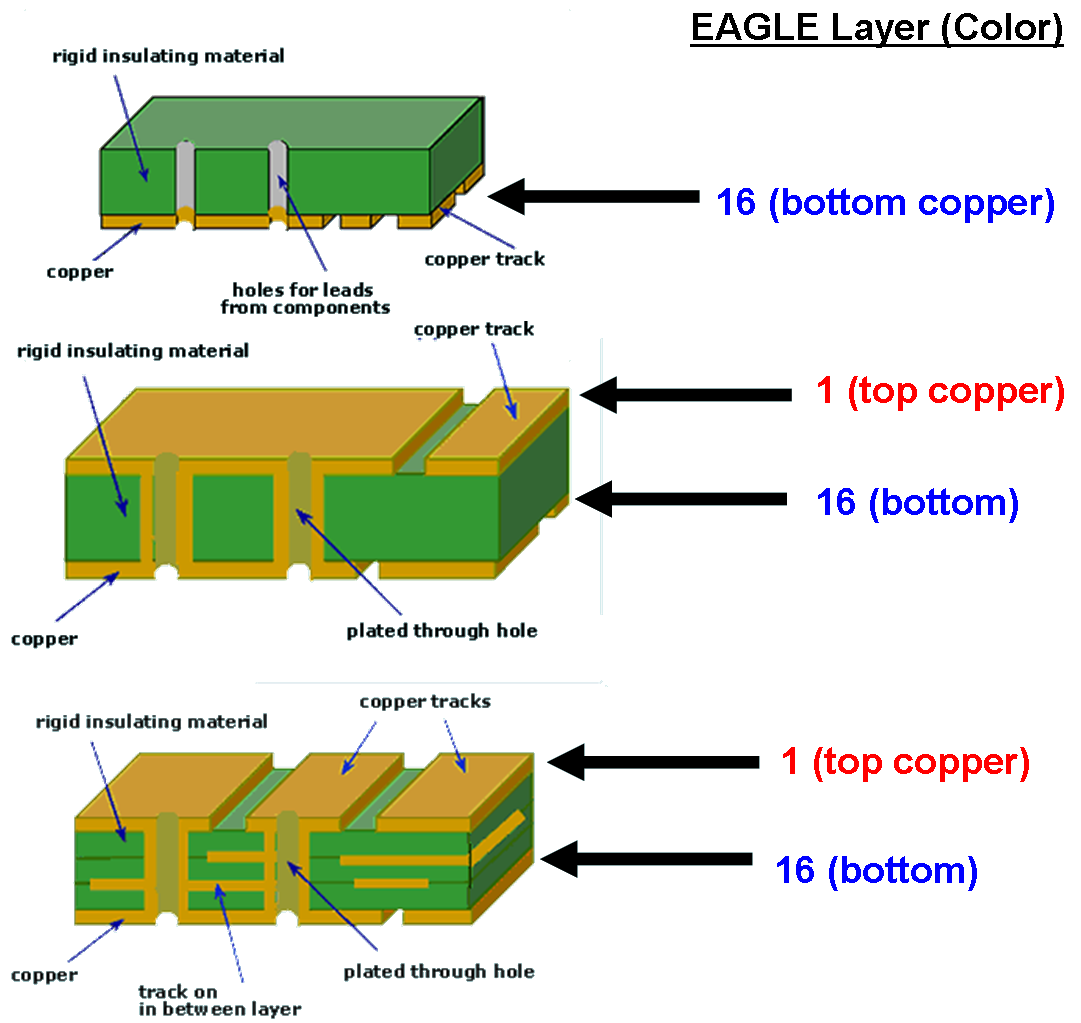
\includegraphics[width=0.7\textwidth]{./fig/PCBLayers}   
\caption[Layered structure of \glspl{PCB}.]{Layered structure of \glspl{PCB}. Top: 1 layer. Middle: 2 layers. Bottom: 4 layers. Source: \cite{online:pcblayers}}   
\label{fig:pcblayers}                                                       
\end{figure}  

A \gls{PCB} basically consists out of copper layers, substrate layers and vias to interconnect different layers (cf. fig. \ref{fig:pcblayers}). There are three different kind of vias in modern electronics:
\begin{enumerate}
\item Through-hole vias as one can see in fig. \ref{fig:pcblayers}
\item Blind vias, which only connect an outer layer to one (or multiple) inner layers
\item Buried vias, which connect two copper layers inside
\end{enumerate}
Blind and buried vias can be implemented as micro vias, which means nothing, but that they are very small, because a laser is used to melt two layers together in a tiny (\ensuremath{<} \SI{0.1}{\milli\metre}) circular area. Conventional \gls{DIY} etching techniques only support the first option. The other two options are usually nowadays still more expensive than normal through-hole vias, which have been around for quite some time already.  Without reservations, using a \gls{DIY} approach, \glspl{PCB} with a complexity of two layers can be crafted nowadays. The basic idea of \gls{DIY} \gls{PCB} crafting is to remove the copper from a blank in certain areas to obtain the desired layout. Distributors nowadays offer blanks with one or two layers and substrate (with a thickness of usually \SI{1.6}{\milli\metre}). Most common is the format \SI{100}{\milli\metre} x \SI{160}{\milli\metre} (\myemph{Eurocard}). Taking away the copper can be achieved mechanically and chemically, whereas this work is about the latter.  
\newpar
\gls{DIY} etching is usually done in either of two ways: 
\begin{enumerate}
\item The toner transfer method: The layout is printed on glossy or transparent paper and the toner is transfered with heat to the blank copper board (cf. \cite{online:instructtoner}). There are several severe disadvantages with this method e.g. that it is hard to align the masks for a \gls{PCB} with two layers.  
\item The photoresist method: Photoresist is used to cover the copper completely and then a \gls{UV} lamp in combination with a mask printed on transparency is leveraged to destroy the photoresist, where it is not covered by the black color on the transparency (cf. \cite{online:instructphoto}). The cracked photoresist, which is damaged by \gls{UV} light can then be washed away with sodium hydroxid (NaOH). 
\end{enumerate}
In both cases an etching bath is necessary to etch away the unprotected copper. Popular chemicals to achieve the copper removal are iron(III) chloride ($\text{FeCl}_3$) and sodium persulfate ($\text{Na}_2\text{S}_2\text{O}_8$).
\newpar
Sodium persulfate gives better results i.e. better or finer contours. Moreover, the sodium persulfate etching liquid is transparent blue unlike the liquid with iron(III) chloride, which is brown and non-transparent. Solving sodium persulfate in water results in
\begin{center}
	\ch{Na2S2O8_{(s)} -> 2 Na^{+}_{(aq)} + S2O8^{2-}_{(aq)}}.
\end{center}
In the etching process elemental copper is oxidated to copper ions, which are then a part of the etching liquid. 
\begin{center}
	\ch{S2O8^{2-}_{(aq)} + Cu_{(s)} -> 2 SO4^{2-}_{(aq)} + Cu^{2+}_{(aq)}}
\end{center}
Special care needs to be taken of the etching liquid afterwards. Copper ions are toxic for all kind of organisms. The last step of \gls{PCB} crafting is the drilling. It can be challenging especially if one uses small via sizes (down to \SI{0.2}{\milli\metre} is not uncommon). One also has to find solution or rather keep in mind, that a via is supposed to interconnect different \gls{PCB} layers, which is hard to achieve creating \gls{PCB} in a \gls{DIY} manner as one somehow has to plate the inside of the cylindric via drill hole with copper in order to create a genuine via.   
% Write what we opt to achieve with this project.
\newpar 
The goal of this project is to develop cheap and easy-to-use etching equipment for the photoresist method. It shall be very easy for engineers to replicate the equipment and also to even tailor it. All the design files shall be open and available on the net. 
\newpar
In principle, what is necessary to start crafting prototypes, is an etching tank and a \gls{UV} light source. Both are subject to what this project opts to achieve as a result.   
\newpar 
The whole project is pushed regularly on \myemph{Github}: \href{https://github.com/m3x1m0m/EmbeddedEtcher}{https://github.com/m3x1m0m/EmbeddedEtcher}

%%%%%%%%%%%%%%%%%%%%%%%%%%%%%%%%%%%%%%%%%%%%%%%%%%%%%%%%%%%%%%%%%%%%%%%%%%%%%%%%%%%%%%
% Background and Analysis
%%%%%%%%%%%%%%%%%%%%%%%%%%%%%%%%%%%%%%%%%%%%%%%%%%%%%%%%%%%%%%%%%%%%%%%%%%%%%%%%%%%%%%

%%%%%%%%%%%%%%%%%%%%%%%%%%%%%%%%%%%%%%%%%%%%%%%%%%%%%%%%%%%%%%%%%%%%%%%%%%%%%%%%%%%%%%
%% Author:      Nils Weber and Maximilian Stiefel
%% Date:        23.12.2017
%% University:  Uppsala Universitet
%% Department:  Institutionen för informationsteknologi 
%% Course:      Embedded Control System Project
%% Project:     PRECISELY CONTROLLED DIY ETCHING MACHINE 
%%				FOR USAGE AT HOME AND IN SMALL LABS
%%%%%%%%%%%%%%%%%%%%%%%%%%%%%%%%%%%%%%%%%%%%%%%%%%%%%%%%%%%%%%%%%%%%%%%%%%%%%%%%%%%%%%

\chapter{Background and Analysis}
\label{chap:background}
% Talk about papers and available technology. Also put the results of the small market analysis here. 

\section{Market analysis}
\label{sec:marketanalysis}
% Homemade: http://sfprime.net/pcb-etching/
% Market-Overview 
% Bath ~500$: https://goo.gl/8ebNsr
% UV illuminator ~400$:
% https://www.ebay.com/itm/Uv-Licht-Hartende-Maschine-Tragbare-Neue-2Kw-F/232345844072?hash=item3618e43968:g:5c0AAOSwa~BYVNiV
There are already different commercial and non-commercial solutions on the market to realize small-scale \gls{PCB} etching. To find possible problems and optimization potential, in order to create a superior product, a small market analysis (see tab. \ref{tab:marketanalysis}) has been carried out in the in the run-up to the development phase of the project. 

\begin{table}[H]
\centering 
\begin{tabular}{p{0.25\textwidth} p{0.2\textwidth} p{0.15\textwidth} 
p{0.35\textwidth} } 
\textbf{Product}&
\textbf{Distributor / Manufacturer}&
\textbf{Price}& 
\textbf{Technical Data}\\\hline

\specialcell[t]{
AETZGERAET 1\\
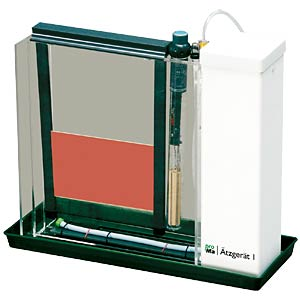
\includegraphics[width=0.15\textwidth]{./fig/etching_machine_2}
}&
Reichelt / PROMA&
129.50 EUR (03.01.2018)&
Needed Acid Volume: 1.75 l. Max. PCB Size: 235 mm x 170 mm. Heating Power: 100 W. Air Pumping System included.\\ 

\specialcell[t]{
500-004 Universal Tank\\
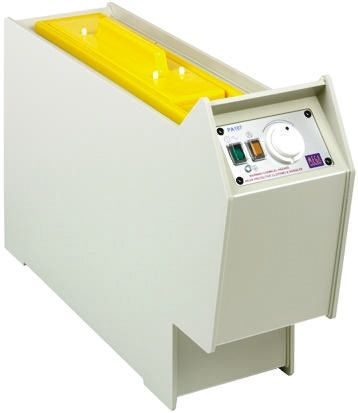
\includegraphics[width=0.15\textwidth]{./fig/etching_machine_1}
}&
RS Components / Mega Electronics&
234.26 GBP (03.01.2018)&
Needed Acid Volume: 5 l. Max. PCB Size: 315 mm x 260 mm. Air Pumping System included\\\hline

\specialcell[t]{
UV-BELICHTER 1\\
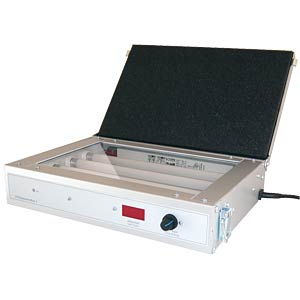
\includegraphics[width=0.15\textwidth]{./fig/uv_light_1}
}&
Reichelt / PROMA&
219.7 EUR (03.01.2018)&
Timer included (0 - 100 min). Max. PCB Size: 160 mm x 250 mm. 4 x 8 W \gls{UV} tubes. Aluminium housing.\\

\specialcell[t]{
UV Exposure Unit\\
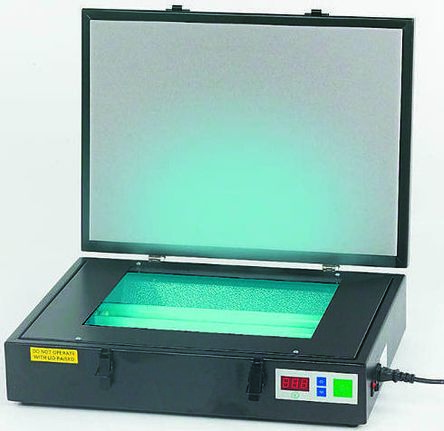
\includegraphics[width=0.15\textwidth]{./fig/uv_light_2}
}&
RS Components / Mega Electronics&
183.32 GBP (03.01.2018)&
Timer included (0 - 6 min). Max. PCB Size: 150 mm x 245 mm. 2 x 8 W \gls{UV} tubes. Metal housing.\\

\hline
\end{tabular}
\caption{Market analysis.}
\label{tab:marketanalysis}
\end{table}

Talking about the etching machines, it is a fact, that all of them do have a heater and some sort of pump to accelerate the chemical reaction introduced in chapter \ref{chap:introduction}. 
\newpar
The \myemph{500-004 Universal Tank} from \myemph{RS Components} is quite big, usually too big for small scale production. For the etching process with sodium persulfate one uses \SI{220}{\gram\per\litre} with \SI{45}{\celsius} (cf. \cite{online:aetzen}). Using the tank from RS Components one needs \SI{1.1}{\kilo\gram} of sodium persulfate, which is neither really practical nor cheap, in case one only wants to etch a few \glspl{PCB} to e.g. test a microstrip bandpass filter. Nevertheless, the design looks really robust and justifies somehow the tough price. Also the maximum \gls{PCB} size is enormous or rather a bit too big for prototyping.
\newpar
The \myemph{AETZGERAET 1} from \myemph{Reichelt} has a way more competitive price, than its equivalent from \myemph{RS Components}. It also seems to be a bit more bodge. The maximum \gls{PCB} size is still impressive as well as the heater power. 
\newpar
Presumably, there is not really a sophisticated control mechanism keeping the temperature close to the setpoint. As far as one can derive this from the given technical data, the thermostats of both devices are based on a bimetal.
\newpar
The \gls{UV} lights are both functioning with \gls{UV} fluorescent tubes. Fluorescent tubes are considered hazardous as they contain mercury vapor, which is extremely toxic (cf. \cite{online:tubes}). For this reason there are plans to ban them in the European Union. It also seems, that one pays for the \gls{UV} light power (number of tubes).
\newpar
Both \gls{UV} light exposure machines have a timer to set the exposure time. This is clearly an important and necessary feature for such a machine as the development process parameters define the quality of the final etched result. Hence, the \gls{UV} light exposure time is an important factor to fine tune the etching result. 
\newpar
Two features neither the \myemph{UV Exposure Unit} from \myemph{RS Components} nor the \myemph{UV-BELICHTER 1} have: It is not possible to adjust the light intensity and the light does only come from one direction at a time. The second shortcoming can introduce problems, since one has to turn on the light, turn it off, turn the \gls{PCB} around and repeat the exposure process. Worst-case, this might lead to alignment problems (e.g. a mounting hole on one side does not align with a mounting hole on the other side). 
\newpar
The exposure units are both relatively pricey, which might be related to the metal housing. 
\newpar
To summarize one can name some ideas how to rectify shortcomings of the currently available products for prototype \gls{PCB} etching: 
\begin{itemize}
\item The etching tank shall not be bigger than \SI{2}{\litre}, as one needs more etching liquid, which is unnecessary for small-scale production. 
\item No expensive metal housings. 
\item It shall be possible, that the user or replicator picks the heater and the compressor for air bubbles flexibly. 
\item No mercury. 
\item Double-sided \gls{UV} light exposure.
\item Precisely controlled light intensity. 
\item Digital and elegant user interface. 
\end{itemize}

\section{LED Drivers}
\label{sec:leddrivers}

\subsection{Buck Converters}
\label{subsec:buck_conv}

\begin{figure}[H]                                                         
\centering          
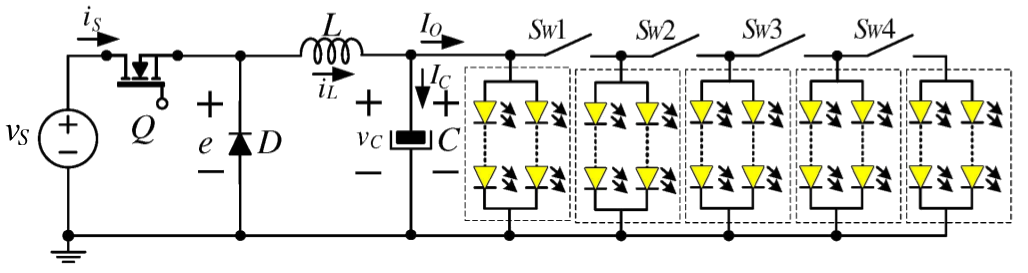
\includegraphics[width=0.7\textwidth]{./fig/buck1}   
\caption[Typcial buck converter as it can be found in a car.]{Typcial buck converter as it can be found in a car. Source: \cite{conference:buck1}.}   
\label{fig:buck1}                                                       
\end{figure}  

One of the ideas for improvements mentioned in section \ref{sec:marketanalysis} induces the use of \glspl{LED}. Therefore, in this section different state-of-the-art \gls{LED} driving techniques are introduced. To drive one \gls{LED} or a string of \glspl{LED} coupled in series one needs to keep the current constant for achieving constant light intensity. It is a well-known fact, that every single \gls{LED} differs concerning its electrical characteristics. The input to output transmission behavior i.e. \ensuremath{I(U)} differs from \gls{LED} to \gls{LED}. This is one challenge one has to master building a \gls{LED} driver. 
\newpar
A common approach, which is popular in automotive applications is a \myemph{buck converter} (cf. \cite{conference:buck1}). \myemph{Buck converters} leverage a switching-frequency to convert a high voltage into a lower voltage. In fig. \ref{fig:buck1} one can see, that in a car the current, which is drawn by the source can change rapidly, as for instance a rear light or an indicator is switched on. For this reason, a controller is needed to ensure, that enough current is provided even if rear light and indicator are switched on simultaneously. Buck converters are that popular because of their remarkable efficiency (greater than 90 \% is normal).
\newpar 
A buck converter from an electrical point of view switches between two states i.e. transistor \myemph{Q} is conducting (1) or non-conducting (2): 
\begin{enumerate}
\item If \myemph{Q} conducts \myemph{L} is directly connected to the voltage source. \myemph{C} and the load is connected to \myemph{L}. The energy stored in \myemph{L} increases. The current change results in a voltage across \myemph{L}, that counteracts the voltage of the source. This of course reduces the voltage over the load. 
\item If \myemph{Q} does not conduct \myemph{D} becomes conductive, because \myemph{L} is now a voltage source. The energy stored in the coil provides a current through the load. \myemph{L} discharges and the voltage across \myemph{L} drops again. The current through the load is still maintained. \myemph{C} helps to keep voltage and current through the load stable (close to \gls{DC} although a certain ripple is normal).  
\end{enumerate}
If the coil is charged and discharged quickly enough one can get into a steady state, where the output is within a certain range. The voltage is ramping up to a maximum and ramping down to a minimum. The output and possible input filters take care of converting this signal to a \gls{DC} signal. 
\newpar
One can also see the buck converter as a low-pass filter connected to a source with a square wave signal. The low-pass filter has ideally a cut-off frequency very close to \SI{0}{\Hz}. The filter excitation happens with a \gls{PWM} signal. One can easily explain how the steering of the current or voltage respectively works looking at the Fourier transformation of a rectangular pulse with a pulse width of \ensuremath{2\,t_0}. The pulse is defined as 
\begin{equation}
    x(t) = \begin{cases}
               1               & -t_0 \leq t \leq t_0\\
               0               & \text{otherwise}
           \end{cases}
\end{equation}
This function can be brought into the frequency domain using the most known equation of the heritage of Joseph Fourier. 
\begin{equation}
X(\omega) = \int_{-\infty}^{\infty} x(t) \cdot e^{-j \omega t} = \int_{-t_0}^{t_0} 1 \cdot e^{-j \omega t}
\end{equation}
Using \ensuremath{\int e^{at} = \frac{1}{a} e^{at}} leads to 
\begin{equation}
X(\omega) = \frac{1}{-j \omega} \, \bigl[ e^{-j \omega t_0} -  e^{j \omega t} \bigr] \text{ .}
\end{equation}
As the next step Euler's formula can be applied.
\begin{equation}
X(\omega) = \frac{2 sin(\omega t_0)}{\omega}  = \frac{2 t_0}{\omega} \frac{sin(\omega t_0)}{\omega t_0} = 2 si(\omega t_0)
\end{equation}
So what one ends up with the sinc function. As one tries to filter out every frequency except of \SI{0}{\Hz}, one can take a close look at \ensuremath{\omega = 0} with the help of l'H\^{o}spital's rule. 
\begin{equation}
\lim_{\omega \to 0} X(\omega) = \lim_{\omega \to 0} \frac{2 sin(\omega t_0)}{\omega} = \lim_{\omega \to 0} 2\,t_0\,cos(\omega t_0) = 2\,t_0  
\end{equation}
Hence, the absolute value of \ensuremath{X(\omega = 0)} becomes larger if the pulse length \ensuremath{t_0} becomes wider. This is why \gls{PWM} steering works. 

\begin{figure}[H]                                                         
\centering          
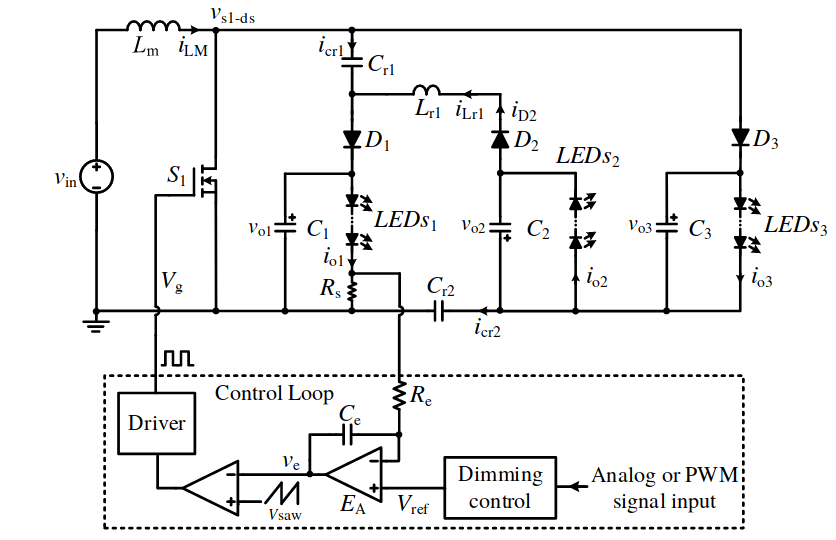
\includegraphics[width=0.7\textwidth]{./fig/buck2}   
\caption[More complex buck converter for automotive applications with analog control circuit.]{More complex buck converter for automotive applications with analog control circuit. Source: \cite{article:buck2}.}   
\label{fig:buck2}                                                       
\end{figure}  

In fig. \ref{fig:buck2} one can see a more complex draft of a buck converter with a analog controller. This circuit originates from \cite{article:buck2}. The first amplifier of the controller is an integrator. It adds memory to the control circuit. It also achieves, that the steering signal is somewhat proportional to the setpoint, which is what one can see analyzing the behavior: 
\begin{equation}
	V_e = - \frac{V_{ref}}{C_e R_e} \int V_{in} \, dt + A 
\end{equation}
whereas \ensuremath{A} is some constant. \ensuremath{V_{in} = R_s \cdot i_{o1}} is according to Ohm's law proportional to the current through the load (and a shunt resistor). The output of the first amplifier is fed into the second stage, a comparator. It compares the input with a sawtooth signal, which results in a \gls{PWM} with a duty cycle depending on the output of the first integrator. As the circuit analysis shows one deals with a proportional-integral controller here.   
\newpar 
Despite their tremendously superior efficiency, there are some disadvantages with buck converters like the switching frequency, that can cause \gls{EMI} problems. Comparing the different possibilities of buck converters one thing also becomes quite clear: Buck converters are complex. Moreover, they always need magnetic devices. Hence, designs become bulkier, less tightly integrated and more expensive if buck converters are used unnecessarily in places where they do not belong. For this reasons, linear regulators still have the right of existence nowadays. 

\subsection{Linear Regulators}
\label{subsec:buck_conv}

\begin{figure}[H]                                                         
\centering          
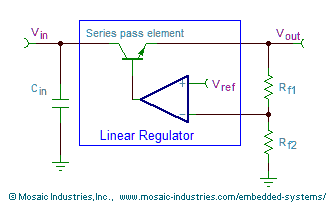
\includegraphics[width=0.4\textwidth]{./fig/linreg1}   
\caption[Typical linear regulator circuit.]{Typical linear regulator circuit. Source: \cite{online:linreg1}.}   
\label{fig:linreg1}
\end{figure}  

The other class of \gls{LED} drivers (power regulators) are linear regulators, which simply adjust their resistance in order to provide a constant current or voltage respectively. Unfortunately, a resistor converts electrical energy into heat, which is why linear regulators suffer from inefficiency, yet, they are very simple and one gets rid of possible \gls{EMI} problems caused by the switching frequency, that buck converters need. In fig. \ref{fig:linreg1} one can see a typical circuit of a linear regulator to provide a fixed voltage for a varying load impedance. This is a pure proportional controller.  

\section{Temperature Control}
\label{sec:temperatureControl}
Two approaches have been considered. Resources here can be money and time spent during development or operation.
\begin{enumerate}
\item Put more resources in sensors and save resources in the system model.
\item Put more resources in the controller model put save resources for sensors.
\end{enumerate}
The first approach was largely inspired by \cite{article:revLag}, where the application of the reversed lag principles are discussed for on-off control. A typical on-off control would result in cyclic temperature fluctuations like shown in fig. \ref{fig:waveforms}.

\begin{figure}[H]
\centering          
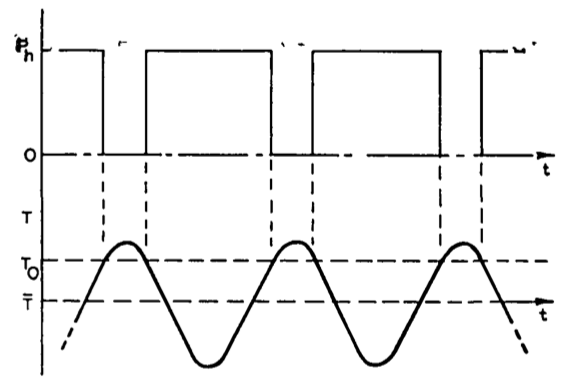
\includegraphics[width=0.4\textwidth]{./fig/waveforms} \caption[Waveforms of heating power and temperature of a system with on-off control.]{Waveforms of heating power and temperature of a system with on-off control. Source: \cite{article:revLag}.}   
\label{fig:waveforms}
\end{figure}  

The paper shows that such a system can be improved by using two control elements which are completely immersed in the fluid of the enclosure. Thus, they are not affected by different errors. One of the two output signals has to have a lagging phase angle, which can be achieved by enclosing it "within a structure which ensures that its mean temperature is that of the fluid, but thermal transmission through the structure introduces a phase lag into the fluctuating component of the temperature of the element" \cite{article:revLag}. However, the circuitry of both sensors results in a leading phase angle of the enclosed sensor with respect to the directly immersed sensor. Thus, the next temperature can be "forseen" without the need of a system model. The paper concludes that "the principle of reversed lag can be applied to an on-off temperature-control system with useful but not spectacular reductions in the amplitude of the cyclic fluctuation in temperature" \cite{article:revLag}. Furthermore, two sensors would need to be purchased to acquire essentially the same data point, which spends more resources and thus contradicts the idea of a low-cost \gls{DIY} solution for small labs or at home.
\newpar
On-off controllers are known for their energy efficiency of their output systems, compared to amplifiers. That is especially true for high power control signals. Electro-heating systems, like the here considered system, are an example for such a system, which is characterized by large time constants. That lowers the need for high frequencies to keep proper parameters of the controlled signal further. The system's dynamics can be approximated with the following equation, where, \(k\) is the static gain, \(L\) is the time delay constant and \(T\) is the system time constant \cite{article:onoffPLC}.
\begin{align}
G(s)=\frac{ke^{-sL}}{1+sT}
\end{align}
A simple on-off controller leaves an static error, which can be reduced by increase of the controller hysteresis. However, this results in increasing the amplitude and period of the oscillation of the controlled signal. This is the disadvantage of this approach. 

The paper \cite{article:onoffPLC} further introduces an inertia corrector, to counteract the described disadvantage. "The hysteresis \(h\) of the controller is the only parameter that can affect the control quality in the basic control system." The new system model with inertia correction is shown in fig. \ref{fig:inertiaCorrection}. If the time constant of the inertia correction is much smaller than the time constant of the system, "then the controller with connected corrector exhibits features of proportional-derivative controller relative to the mean value of controlled signal" \cite{article:onoffPLC}.

\begin{figure}[H]
\centering          
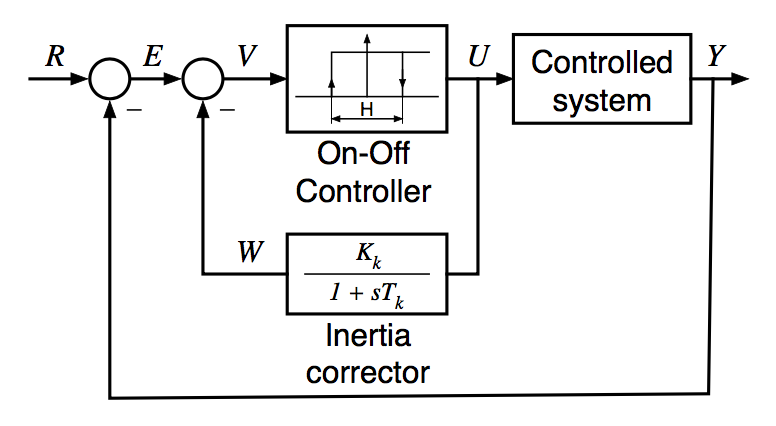
\includegraphics[width=0.4\textwidth]{./fig/inertiaCorrection} \caption[The control system with unity negative feedback and inertia corrector.]{The control system with unity negative feedback and inertia corrector. Source: \cite{article:onoffPLC}.} 
\label{fig:inertiaCorrection}
\end{figure}  

However, as the authors of \cite{article:onoffPLC} show, the steady state error can be eliminated by using an additional corrector, instead of an integrator. This proportional corrector rescales the reference value to the range of 0 to 1, before entering the control comparator. The system has to be pre-identified, but the introduction makes the mean value of the controlled signal independent from any changes of the hysteresis \cite{article:onoffPLC}.

\begin{figure}[H]
\centering          
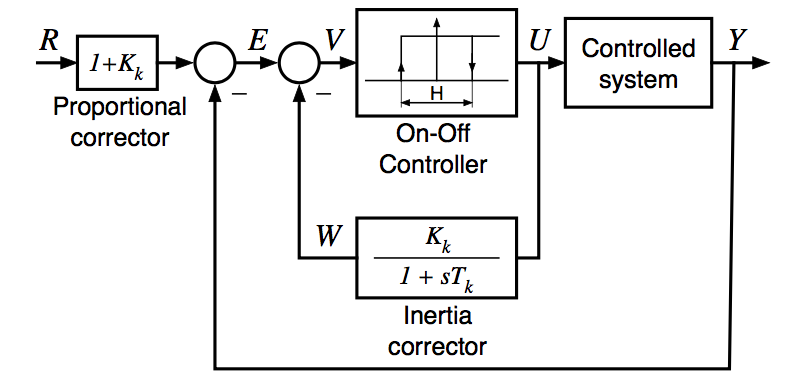
\includegraphics[width=0.4\textwidth]{./fig/inertiaCorrectionProp} \caption[The control system with proportional and inertia correctors.]{The control system with proportional and inertia correctors. Source: \cite{article:onoffPLC}.} 
\label{fig:inertiaCorrectionProp}
\end{figure} 

The paper \cite{article:onoffPLC} concludes that the introduced control system "significantly reduces an amplitude of oscillation of controlled signal and shortens its period. An additional proportional corrector eliminates an error of the mean value of the controlled signal in the steady state."

%%%%%%%%%%%%%%%%%%%%%%%%%%%%%%%%%%%%%%%%%%%%%%%%%%%%%%%%%%%%%%%%%%%%%%%%%%%%%%%%%%%%%%
% Design
%%%%%%%%%%%%%%%%%%%%%%%%%%%%%%%%%%%%%%%%%%%%%%%%%%%%%%%%%%%%%%%%%%%%%%%%%%%%%%%%%%%%%%

%%%%%%%%%%%%%%%%%%%%%%%%%%%%%%%%%%%%%%%%%%%%%%%%%%%%%%%%%%%%%%%%%%%%%%%%%%%%%%%%%%%%%%
%% Author:      Nils Weber and Maximilian Stiefel
%% Date:        23.12.2017
%% University:  Uppsala Universitet
%% Department:  Institutionen för informationsteknologi 
%% Course:      Embedded Control System Project
%% Project:     PRECISELY CONTROLLED DIY ETCHING MACHINE 
%%				FOR USAGE AT HOME AND IN SMALL LABS
%%%%%%%%%%%%%%%%%%%%%%%%%%%%%%%%%%%%%%%%%%%%%%%%%%%%%%%%%%%%%%%%%%%%%%%%%%%%%%%%%%%%%%

\chapter{Design}
\label{chap:design} 
\section{System Architecture and Required Functionality}
\label{sec:system_arch_and_req}
% Explain how our system is build up. 
First, the system consists out of two machines, the \gls{UV} light and the etching tank. Of course, these two machines are different and therefore need different designs. However, effort has been put into trying to use as many software and hardware components in both parts simultaneously to reduce the overall workload.  

\begin{figure}[H]                                                         
\centering          
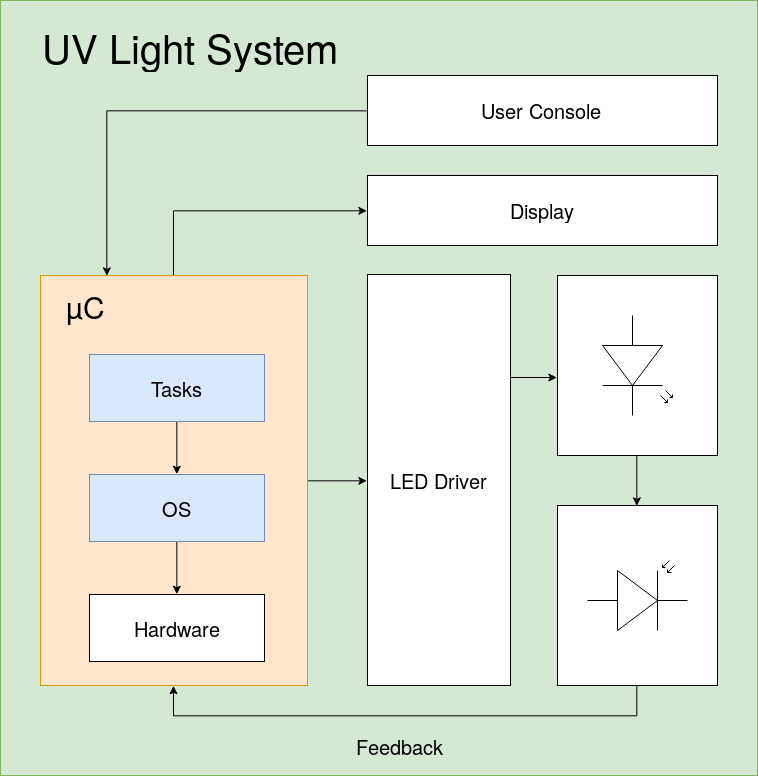
\includegraphics[width=0.5\textwidth]{./fig/uv_light_simple}   
\caption[\mu C with user interface, custom LED driver and feedback loop.]{\mu C on the left executing tasks with an OS below. User interface is hooked up to the \mu C. Custom LED driver is connected to LEDs, steered by software. Feedback comes from a light sensor.}   
\label{fig:uv_light_simple}
\end{figure}  

In fig. \ref{fig:uv_light_simple} a rough sketch of the \gls{UV} light exposure unit is shown. The most important part is probably the \glspl{LED} and the driver for it. A feedback from the \glspl{LED} is generated with the help of a light sensor. This feedback can be coupled into a controller steering the driver. Besides the \gls{LED} driver, one needs a microcontroller, that executes the \gls{OS} and tasks to implement the desired functionality. In addition, some components for communication with the user are necessary, i.e. a console and a display. The user must be able to adjust exposure time and intensity. The intensity is not changeable with devices currently available on the market. 

\begin{figure}[H]                                                         
\centering          
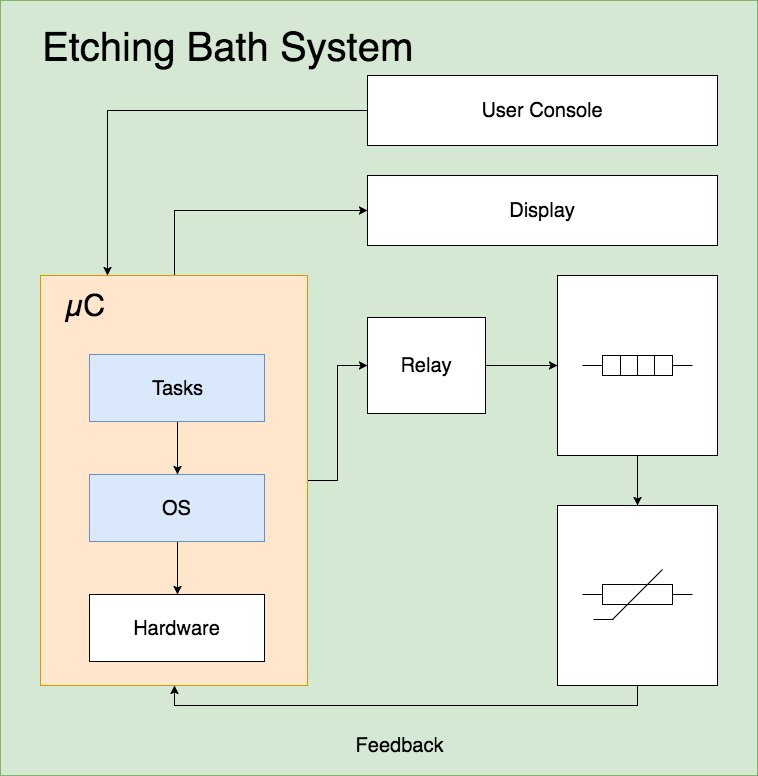
\includegraphics[width=0.5\textwidth]{./fig/etching_bath_simple}   
\caption[\mu C with user interface, heater and feedback loop.]{\mu C on the left executing tasks with an OS below. User interface is hooked up to the \mu C. The heater is connected via a relay, steered by software. Feedback comes from a temperature sensor.}   
\label{fig:etching_bath_simple}
\end{figure} 

In fig. \ref{fig:etching_bath_simple} the system architecture is sketched. Comparing to fig. \ref{fig:uv_light_simple} one can see many similarities, which result from the efforts to keep many parts of the system interchangable. The heater is not very sophisticated, thus the control is realized via a simple, optocoupled relay. An \gls{NTC} resistor is used as a temperature sensor and submersed into the etching bath. Thus, it closes the feedback loop for the control system.

Tab. \ref{tab:design_choices_uv_light} gives a bit more insights dealing with which components have been chosen and why. Also it includes information about the costs of each component. 

\section{Design Choices}
% Explain which design choices have been made and why.

The following table explains why different components have been chosen to enable the required functionality.

\begin{table}[H]
	\centering 
	\begin{tabular}{p{0.2\textwidth} p{0.2\textwidth} p{0.1\textwidth} 
		p{0.4\textwidth} } 
		\textbf{Block} &
		\textbf{Component(s)}&
		\textbf{Costs}& 
		\textbf{Justification of the
		Choice}\\\hline
		Microcontroller &
        STM32 microcontroller family &
        From 1.30 USD & 
        The µCs are cheap, because they are used everywhere. Open-source \glspl{IDE} are available and have a huge community. Open-source hardware is available as well. Big family tree with all kind of options. Powerful ARM Cortex-M0, Cortex-M3, Cortex-M4, Cortex-M7 32-bit processors. Ultra-low power (L-models) available. \\\hline 
        \gls{LED} Driver & 
        Custom designed linear regulator &
        0.40 USD per stage (25.60 USD for 64 stages) &
        One needs less components with a linear regulator (saves space and money). Choosing the voltage supply as close as possible to the voltage drop over the \gls{LED} or the \gls{LED} string, the efficiency is not too bad. Control part becomes very simple, yet effective. \\\hline
        Display &
        \gls{OLED} SSD1306 &
        2.50 USD &
        The display is cheap. Open-source driver software only needs to be ported to the platform. \gls{SPI} and \gls{I2C} interface available. \gls{OLED} technology is very elegant in comparison to alternatives.\\\hline
        User Console &
        Two rotary encoders and one tactile switch & 
        2 USD & 
        Very comfortable interface. One encoder for the exposure time, one for the light intensity and the tactile switch for starting the exposure process.\\
         &
        One rotary encoder including a push button & 
        \(<\) 1 USD & 
        Different parameters of the controller can be changed via the rotary encoder; the button is to switch between changing the parameter value or the parameter.\\\hline 
        Light Sensor &
        TSL2561 &
        1 USD & 
        Very easy to use with \gls{I2C} interface. Integrated amplifier. Very small. No need to develop a readout circuit with a photodiode.\\\hline 
        Temperature Sensor &
        NTCALUG01T103FL &
        3.5 USD & 
        Simple \gls{NTC} in metal package with ring connector. Robust, used in automotive applications. Comes with \SI{150}{\milli\metre} of wire. Detailed support from manufacturer.\\\hline
        Relay with optocoupler &
        - &
        \(<\) 1 USD & 
        Simple and safe to use via digital out.\\\hline 
        Air Temperature Sensor &
        SHT31 &
        4 USD & 
        Highly accurate air temperature and humidity sensor. Includes \gls{I2C}-interface.\\\hline
	\end{tabular}
	\caption{Design choices for the system: Why has each component been chosen?}
	\label{tab:design_choices_uv_light}
\end{table}




\section{Mathematical Model of the Tank}

Using the concept of energy balance to describe the thermodynamical model of the tank yields following equations \cite{online:mathModel}:
\begin{equation*}
Heat_{in} = Heat_{out} + Heat_{stored}
\end{equation*}

\begin{equation}
q_i=\frac{\theta_t - \theta_e}{R_{ta}}+c\frac{d\theta_t}{dt}
\end{equation}

with \(c\) as heat capacity of water, 4184\si{\frac{\joule}{\kilogram\kelvin}}, and
\(R_{ta}\) as temperature resistance between tank and ambient environment.

To further develop a model, different measurements are necessary. Water has a different specific heat capacity in different phases, i.e. as ice or water \cite{online:watercurve}.
\begin{equation}
q=m*C_s*\Delta T
\end{equation}

Different measurements to gather data to further build and understand the mathematical system. All measurements are to be done with the original water tank, heater and the temperature sensor.
\begin{itemize}
\item Cooling behavior 
	\begin{itemize}
	\item Measure temperature every 10s while cooling down water 
	\item Start from different temperatures
	\end{itemize}
\item Heating behavior
	\begin{itemize}
	\item Measure temperature every 10s while heating up water
	\end{itemize}
\item Determine time constants
\end{itemize}







%%%%%%%%%%%%%%%%%%%%%%%%%%%%%%%%%%%%%%%%%%%%%%%%%%%%%%%%%%%%%%%%%%%%%%%%%%%%%%%%%%%%%%
% Implementation
%%%%%%%%%%%%%%%%%%%%%%%%%%%%%%%%%%%%%%%%%%%%%%%%%%%%%%%%%%%%%%%%%%%%%%%%%%%%%%%%%%%%%%

%%%%%%%%%%%%%%%%%%%%%%%%%%%%%%%%%%%%%%%%%%%%%%%%%%%%%%%%%%%%%%%%%%%%%%%%%%%%%%%%%%%%%%
%% Author:      Nils Weber and Maximilian Stiefel
%% Date:        23.12.2017
%% University:  Uppsala Universitet
%% Department:  Institutionen för informationsteknologi 
%% Course:      Embedded Control System Project
%% Project:     PRECISELY CONTROLLED DIY ETCHING MACHINE 
%%				FOR USAGE AT HOME AND IN SMALL LABS
%%%%%%%%%%%%%%%%%%%%%%%%%%%%%%%%%%%%%%%%%%%%%%%%%%%%%%%%%%%%%%%%%%%%%%%%%%%%%%%%%%%%%%

\chapter{Implementation}
\label{chap:implementation}
% Explain explicitly how things have been implemented or are supposed to be implemented i.e. software, hardware, mechanics. 

\section{UV Light}
\label{sec:uv_light}

\begin{figure}[H]                                                         
\centering          
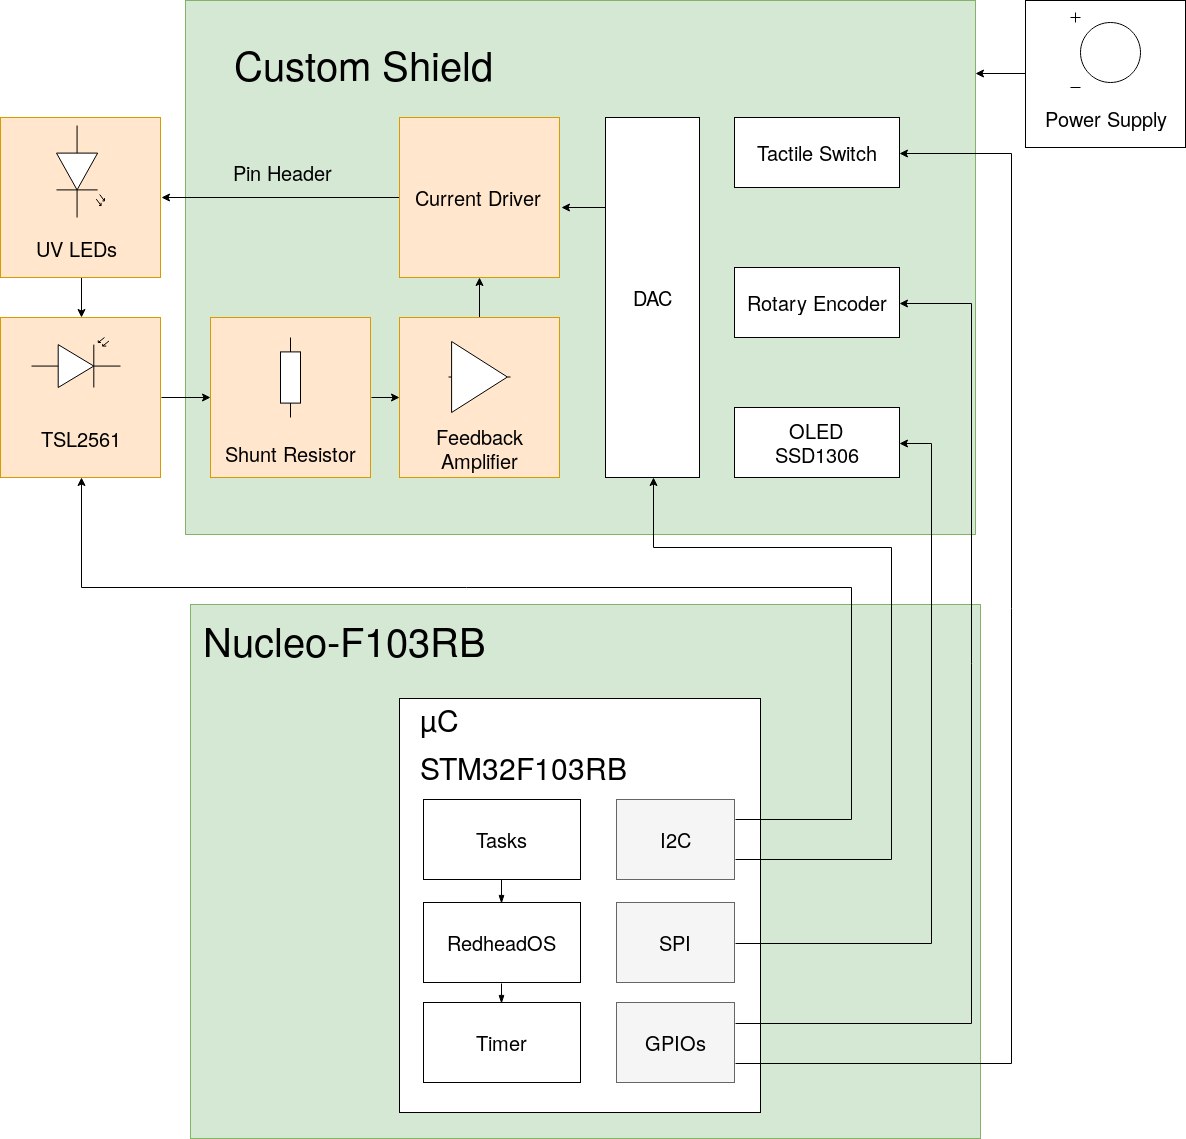
\includegraphics[width=0.8\textwidth]{./fig/uv_light_block_diagram}   
\caption[UV light system.]{UV light system. Top: Custom extension board. Bottom: Nucleo board with custom software.}   
\label{fig:uv_light_block_diagram}                                                       
\end{figure}  

The decision has been made to use the \myemph{Nucleo-F103RB}, a cheap (approx. 25 USD) development board, instead of designing a processor board. This has a couple of advantages:
\begin{itemize}
\item No \gls{PCB} design required to bring the STM32 on a board. 
\item Directly start programming without waiting until the hardware is ready.
\item Debugger and programmer from STM included. 
\item Time to develop something, that works is shortened. 
\end{itemize}
Instead, a custom extension board for the Nucleo board has been designed (cf. fig. \ref{fig:uv_light_block_diagram}). Everything has been laid out so the hardware can drive a lot of \myemph{industry standard T-1 3/4} \SI{5}{\milli\metre} \glspl{LED}. In fact it can supply 256 of these \glspl{LED}. Four \glspl{LED} can be put in series. The voltage drop does not exceed \SI{14}{\volt}. This has been verified by measurements in the lab with a current of \SI{30}{\milli\ampere}. Hence, a power supply of \SI{18}{\volt} is sufficient. Although something closer to \SI{14}{\volt} would be more efficient. However, it does not matter so much, as long as the linear regulator can dissipate enough power without being destroyed. 
\newpar
The \glspl{LED} are meant to be connected with a 64 pin header (low-side) and a 10 pin header to the board. Actually, a rather big housing has been built together to take in the \glspl{LED} and the electronics eventually. 
\newpar 
A small \gls{OS}, developed from scratch, runs on the STM32 to make real-time scheduling possible with a small code footprint and give a programmer all the necessary infrastructure to program conveniently (semaphores, queues, printf etc.). 

\subsection{Hardware}
\label{subsec:uv_light_hw}
\begin{figure}[H]                                                         
\centering          
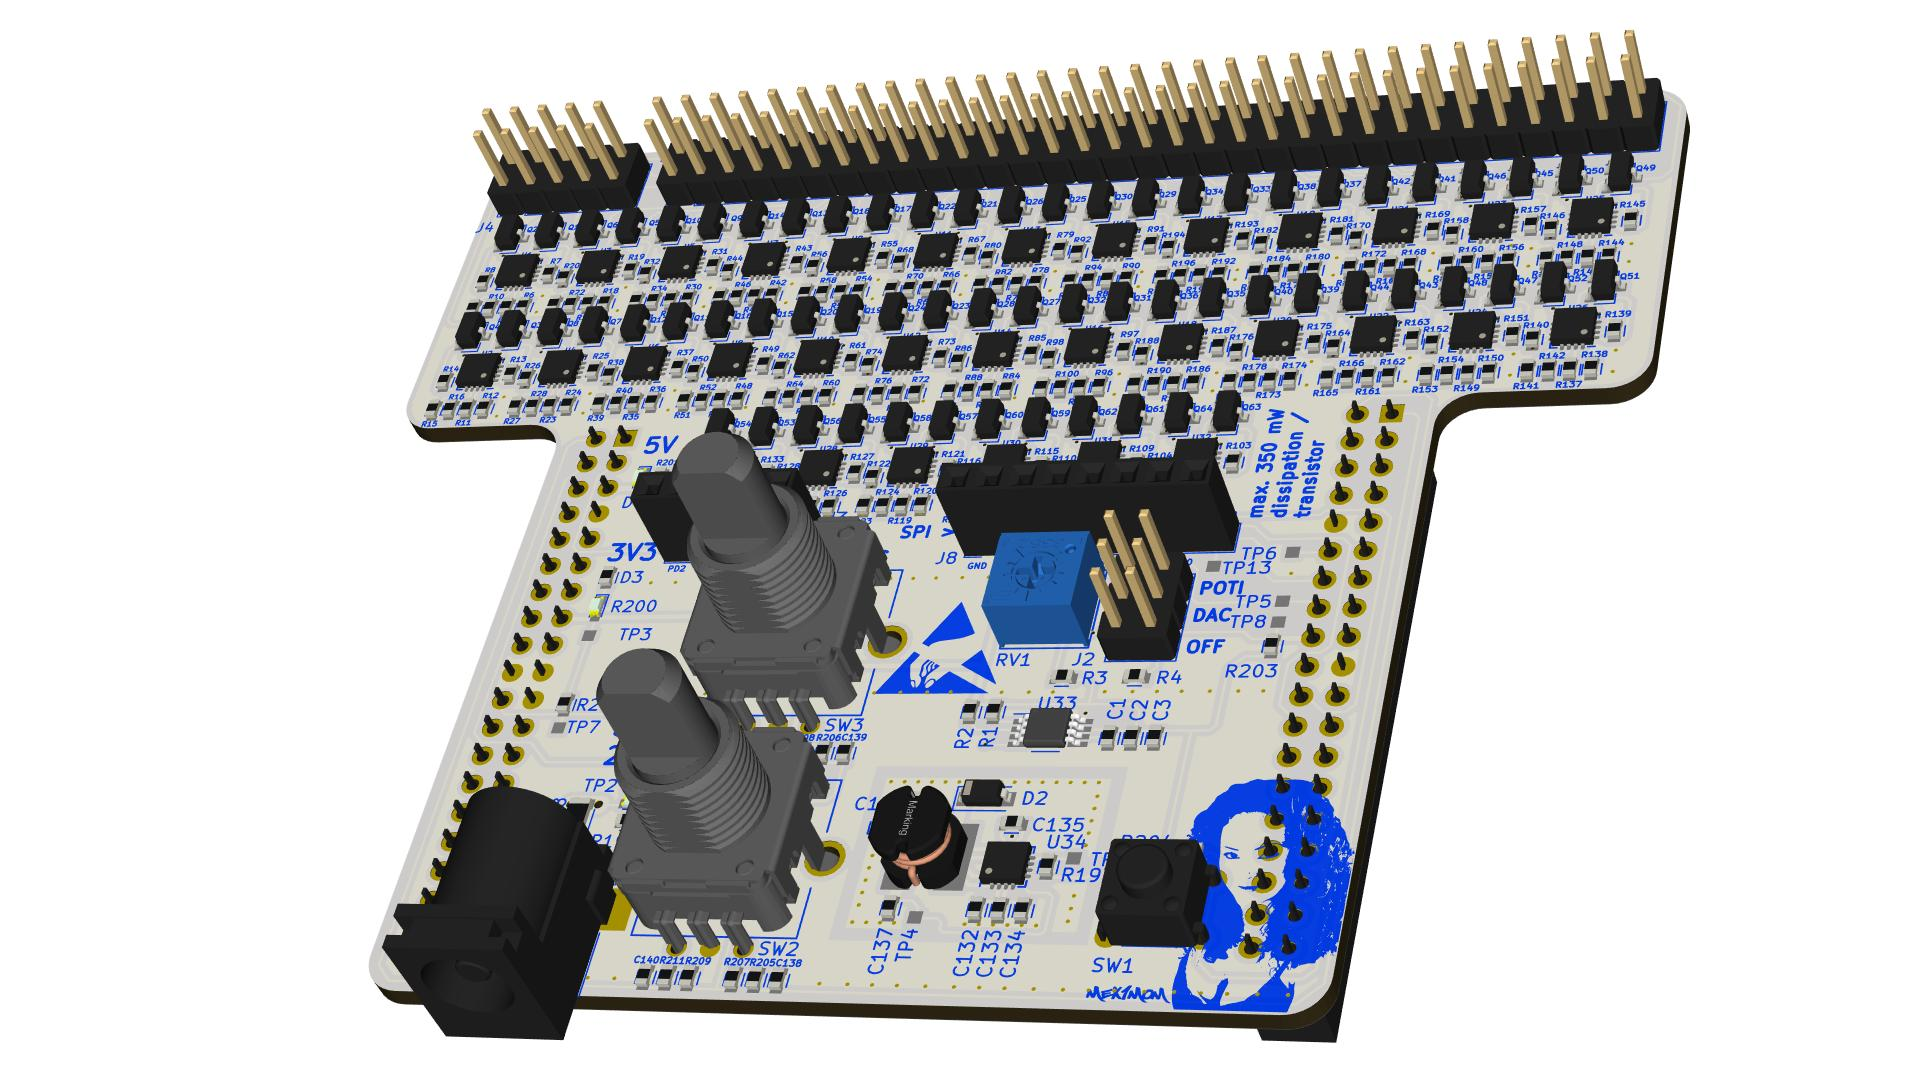
\includegraphics[width=1\textwidth]{./fig/3d_pic_pcb}   
\caption[Four layer extension board for the Nucleo-F103RB.]{Four layer extension board for the Nucleo-F103RB to drive 64 \gls{LED} channels. All 3D models have been entered into the \gls{ECAD} program to prevent unintended surprises.}   
\label{fig:3d_pic_pcb}                                                       
\end{figure}  
The board shown in fig. \ref{fig:3d_pic_pcb} has been developed and produced in the course of this project. It has four layers, but no micro vias, to, on the one hand get a grip on the complexity, and on the other hand save money (micro vias are still expensive than through-hole vias in production, cf. \ref{chap:introduction}). As an introduction, one can briefly list the features of this sophisticated piece of hardware.
\begin{itemize}
\item 64 \gls{LED} driver stages.
\item \SI{6.4}{\ampere} (\SI{0.1}{\ampere} per stage) and \SI{24}{\volt} max. input. 
\item \SI{0.2}{\ampere} max. and \SI{350}{\milli\watt} dissipation max. per stage. Stages can be left floating if unused without the threat of damaging the device. 
\item 10 Bit \gls{DAC} to steer the driver combined with feedback amplification to achieve a tremendously fine resolution. 
\item Optional potentiometer to set the current. 
\item Control loop to guarantee the desired current and respond quickly to changing the setpoint. 
\item 2 rotary encoders and 1 tactile switch.
\item \gls{I2C} header.
\item \gls{SPI} header. 
\end{itemize}

In appendix \ref{append:extension} an extract of the schematics of the board is available. The following lines shall briefly describe the different circuits. One page 1/37 one can see, that there are four main modules: The interface to the processor board, the \gls{LED} driver, the power management and  the user interface. 
\newpar 
On page 2/37 one can see the \gls{LED} driver part. On the right side, the \myemph{DAC101C085} from \myemph{Texas Instruments} is placed. \SI{0}{\ohm} resistors give flexibility in setting the bus address. The reference voltage is connected to the supply voltage of \SI{3.3}{\volt}, provided by the processor board. Below that, one can see a potentiometer and a connector, that can be populated with a jumper to set the reference voltage for the driver accordingly. The reference voltage is translated into a current whereas with the resistor configuration so far \SI{1}{\volt} equals \SI{10}{\milli\ampere}. The last connector on the right side is to make the \gls{I2C} interface 1 of the microcontroller accessible.
On the left side there are 32 times 2 driver stages, which equals a total of 64 driver stages. The group forming is as it is, because the deployed quadruple operational amplifier (\myemph{LM324}) can be used for 2 stages as it has four operational amplifiers inside. In addition, one can see the big 64 pin header for \gls{LED} connection. 
\newpar 
Page 3/37 reveals the \gls{LED} driver design as it shows one driver stage, which consists out of one \myemph{LM324} (four operational amplifiers) and two \myemph{MBT3904} (NPN transistor). The controller works as follows: 
\begin{enumerate}
\item A current \ensuremath{I_C} flows through the transistor into the shunt resistor \ensuremath{R_S}, which is connected to the input of a non-inverting amplifier. 
\item The shunt resistor \ensuremath{R_S} has a small resistance value of \SI{10}{\ohm} and translates the current \ensuremath{I_C} into a voltage \ensuremath{V_S = I_C \cdot R_S}. This might even work with a smaller shunt resistor. 
\item Obviously, the resulting voltage \ensuremath{V_S} is very small, which is why there is an amplifier in the feedback loop. Analyzing this operational amplifier configuration one ends up with the following relation between input and output: 
\begin{equation}
V_{out} = V_{in} \frac{R_1 + R_2}{R_1} = V_{in} \frac{\SI{20}{\kilo\ohm} + \SI{180}{\kilo\ohm}}{\SI{20}{\kilo\ohm}} = 10 V_{in}
\end{equation}
The size of the shunt resistor and the amplification factor determine the mapping between bits set in the \gls{DAC} (10 Bits) and the current through the \gls{LED}. Making the shunt resistor smaller is of course better because of unnecessary heat dissipation, but one has to keep in mind, that the operational amplifier is absolutely low-cost and has a certain offset voltage. Also, the closer one gets to the power supply voltages of the operational amplifier, the more problems of non-linearity occur. 
\item In the last step, the voltage output of the first stage is compared with the setpoint, coming either from the \gls{DAC} or the potentiometer. The output of the second stage is a current \ensuremath{I_B} proportional to the difference between the inputs. 
\begin{equation}
 I_C = I_B \cdot \beta
\end{equation}
is the relation between the base current and the collector current. According to the datasheet \ensuremath{\beta} is somewhere between 100 and 300, which is why a small error is neglected, since \ensuremath{I_C \gg I_B}: The current into the transistor collector is not the same as the current going out of the emitter. Hence, the current through the \glspl{LED} is about less then 1 \% smaller than the current the controller is aware of. 
\end{enumerate} 
The power distribution becomes clear taking a look at page 35/37. Using a barrel jack a lot of standard power supplies can be interfaced with the board. The board design is \myemph{IPC 2221} compliant given the parameters one can see in the schematics. A powerful buck converter \gls{IC} the \myemph{TS30011} steps down the input voltage to \SI{5}{\volt}. The processor board can be powered with external \SI{5}{\volt}, assumed that configured correctly. \SI{3.3}{\volt} can then be obtained from the processor board to supply e.g. the \gls{DAC} or the \gls{OLED} screen on the extension board. 
\newpar 
Page 36/37 shows the interfacing between processor and extension board. Nothing to really see here. 
\newpar 
The small user interface is on the last page 37/37. One connector enables access to the \gls{SPI} 1 of the microcontroller. Also one finds the tactile switch and two rotary encoders, which are debounced hardware wise. 

\subsection{Software}
\label{subsec:uv_light_sw}

\begin{figure}[H]                                                         
\centering          
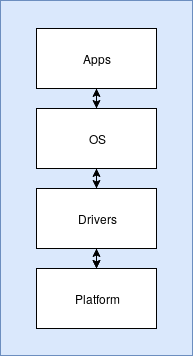
\includegraphics[width=0.3\textwidth]{./fig/layering}   
\caption[Layered code structure]{Layered code structure}   
\label{fig:layering}                                                       
\end{figure}

Fig. \ref{fig:layering} shows how the code ought to be structured in general. This allows to migrate the actual functionality quickly to another platform. However, as it turned out it can be hard sometimes not run into layer breaches i.e. the code one layer is supposed to only communicate with the layer above and the layer below if implemented properly.  
\newpar 
Every kind of controller is implemented in the \myemph{App layer}. The \gls{OS} layer provides a \gls{PID} controller infrastructure. A task is running, which handles the controller for the \gls{UV} light intensity, that gets the feedback input from the light sensor and steers the \gls{DAC}.
\newpar 
The \gls{DAC} driver is implemented in the \myemph{Driver layer}, whereas this driver needs to use \gls{I2C}, which is a hardware component of the \myemph{STM32}. \gls{I2C} is for this reason located in the \myemph{Platform layer}. Switching to another microcontroller, one ideally only needs to change the \myemph{Platform layer}. 
\newpar 
The \gls{OLED} screen driver belongs into the \myemph{Driver layer} accordingly and there are tasks to handle the user input from the rotary encoders and the switch in the \myemph{App layer}.  

\subsection{Mechanics}
\label{subsec:uv_light_mechanics}

\begin{figure}[H]                                                         
\centering          
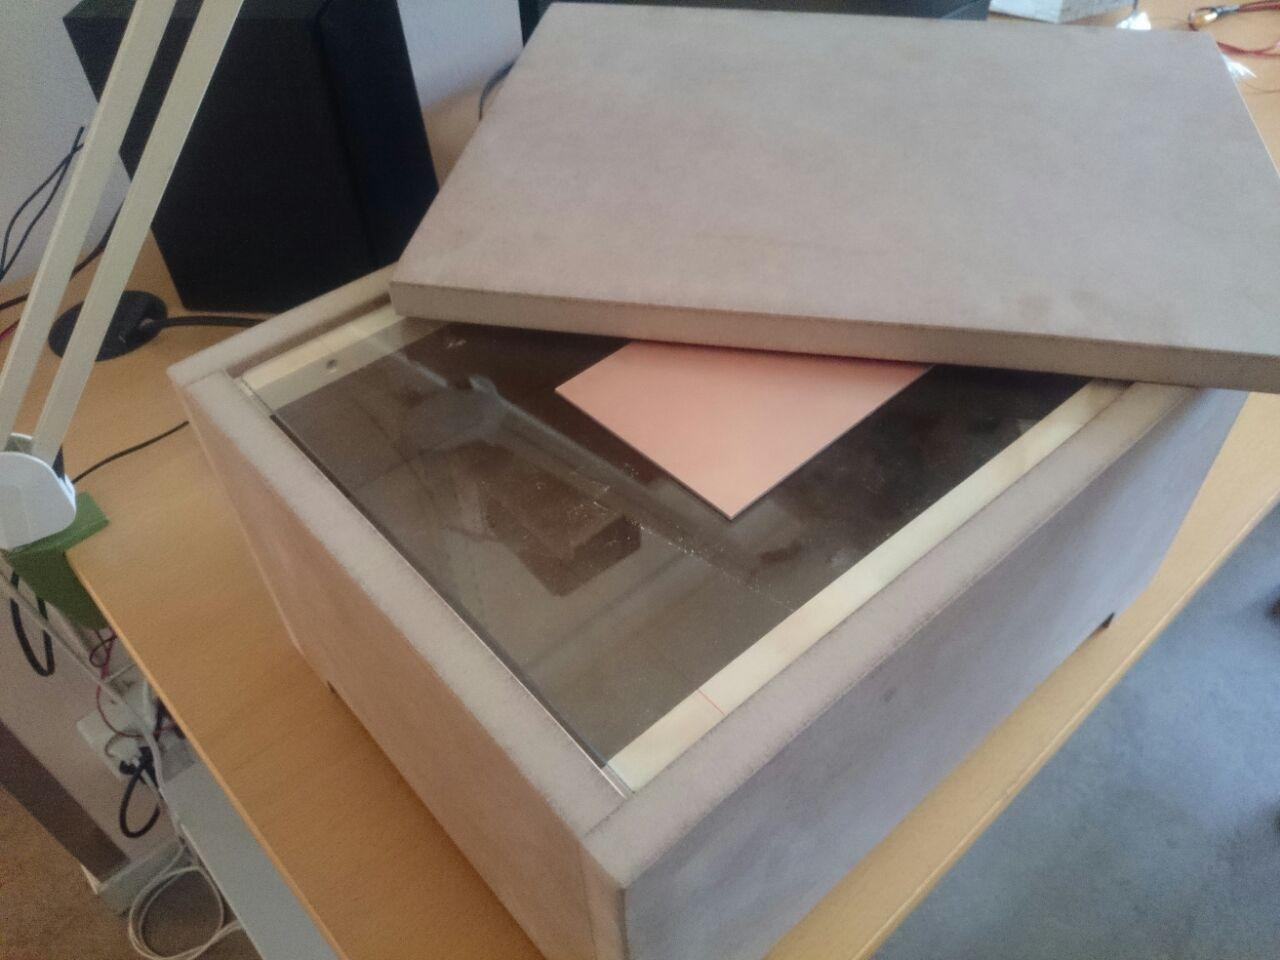
\includegraphics[width=0.6\textwidth]{./fig/uv_lamp_box}   
\caption[Wooden box for the \gls{UV} exposer unit.]{Wooden box for the \gls{UV} exposer unit with 16 x 16 \gls{LED} matrix.}   
\label{fig:uv_lamp_box}                                                       
\end{figure} 

In cooperation with a carpenter a wooden box has been build, which uses a glass plate from an old scanner (cf. fig. \ref{fig:uv_lamp_box}). A wooden plate is located below the glass. On this wood plate there is a matrix out of 256 \glspl{LED}. The distance between glass and \gls{LED} matrix can be varied with the help of IKEA parts, that are plugged into the sidewalls while simultaneously holding the \gls{LED} matrix. The cabling, drilling and soldering to create the \gls{LED} matrix is a nightmare as one can imagine. Each single \gls{LED} needs to be connected to wires to lengthen the legs of it. Subsequently, every \gls{LED} is fixed in a hole and fixed with a hot glue gun. Always four \glspl{LED} have to be connected together in series. Eventually, every single one of the 64 stages has to be connected somehow to the extension board. For this reason a small adapter \gls{PCB} has been constructed (cf. fig. \ref{fig:adapter_board}). This board can be installed with wood screws and high- and low-side of the \glspl{LED} can be soldered. Following, one just has to plug in the two ribbon cables.   

\begin{figure}[H]                                                         
\centering          
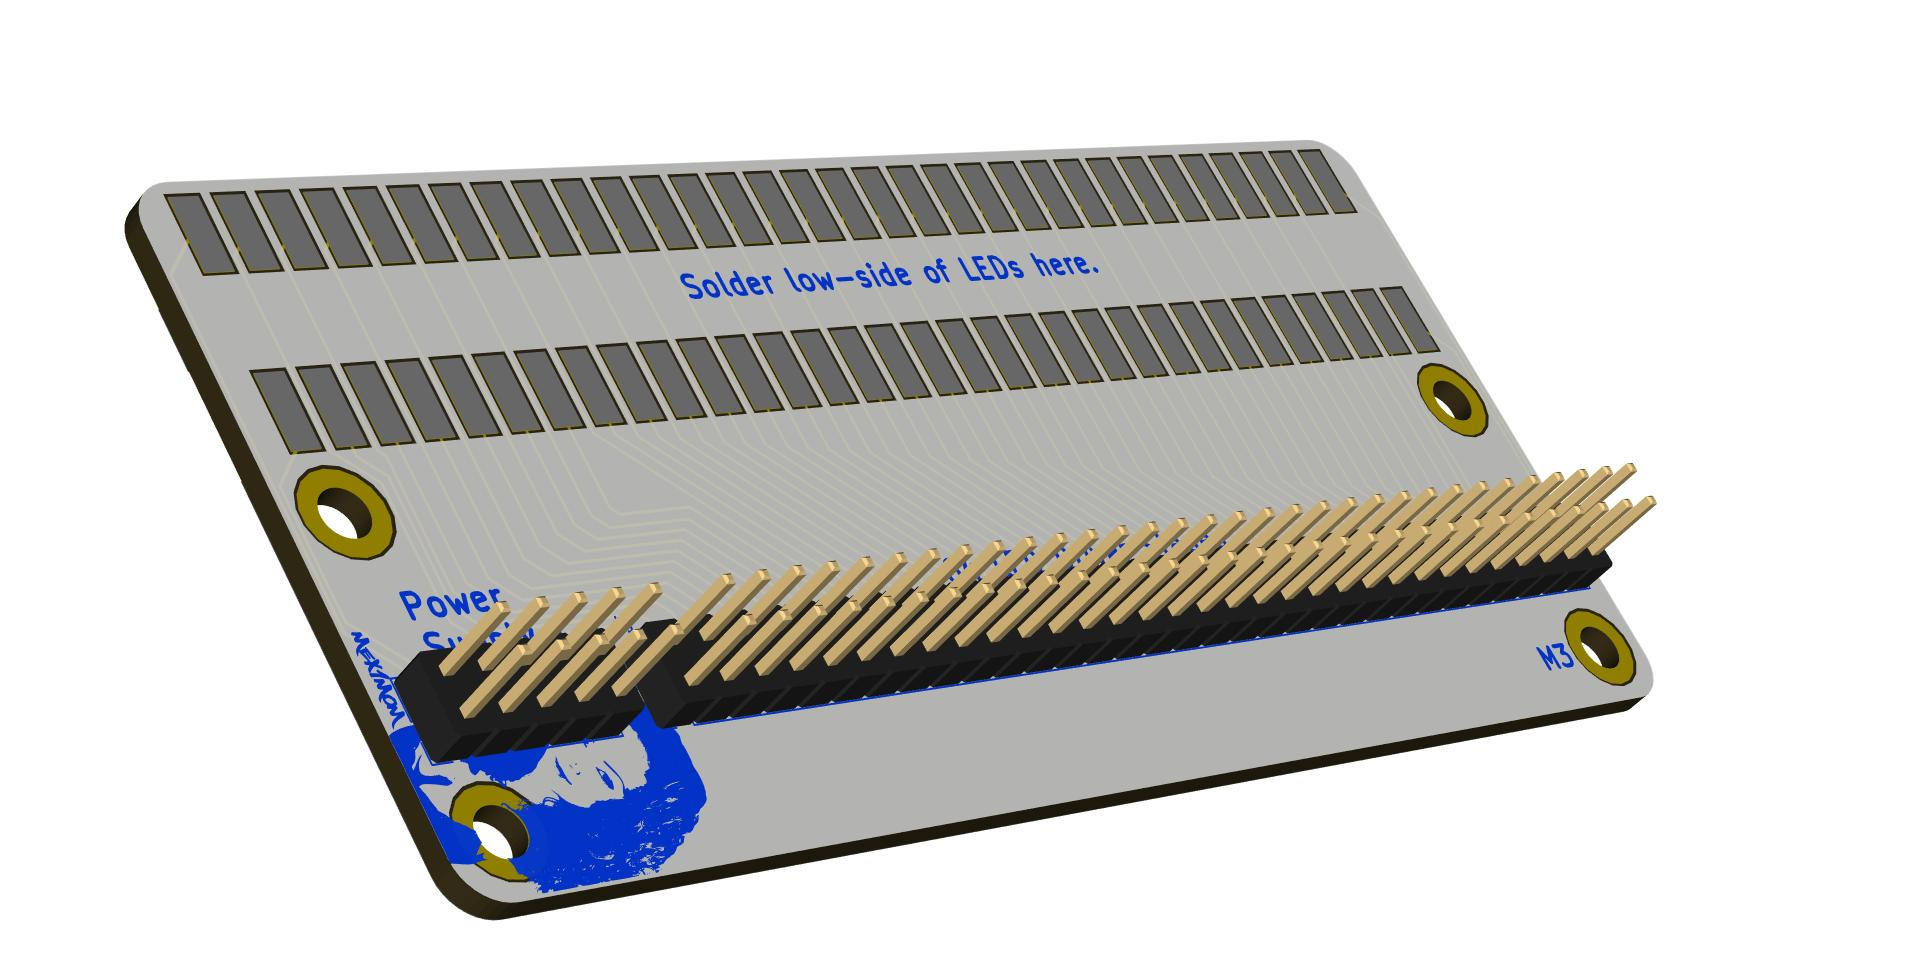
\includegraphics[width=0.8\textwidth]{./fig/3d_pic_2}   
\caption[Adapter board for \gls{LED} matrix enables simple plug and play.]{Adapter board for \gls{LED} matrix enables simple plug and play after soldering high- and low-side of the \gls{LED} strings.}   
\label{fig:adapter_board}                                                       
\end{figure} 


\section{Etching Tank}
\label{sec:etching_tank}
As briefly outlined in section \ref{sec:uv_light}, the Nucleo-F103RB has been chosen. During the development of the temperature control the Nucleo-L073RZ has been used for the simple reason of immediate availability. This led to more complications that originally anticipated, as discussed later in chapter \ref{chap:evaluation}.

\subsection{Hardware}
\label{subsec:etching_tank_hw}
Less sophisticated is the electric hardware for the temperature control, as it is in early prototyping stage to date and future tests will provide knowledge to chose the smartest path in further developments.
As shown earlier in fig. \ref{fig:etching_bath_simple} the system output is a 50W heater which is controlled via a relay. Its power source is a common power outlet of 230VAC. This relay is optocoupled to a normal digital output GPIO for security reasons.
For the user interface a small OLED screen with the SSD1306 driver and I2C interface is used as output, and a rotary encoder is used as input. The screen shows the temperature inside the etching bath, the reference temperature and the ambient temperature.
Since no cooling mechanism is installed, the reference temperature cannot be set below the ambient temperature.

\subsection{Software}
\label{subsec:etching_tank_sw}
Core of the system is the control algorithm implemented as described in \cite{article:onoffPLC}. The algorithm shown in fig. \ref{fig:inertiaCorrectionProp} has been implemented in \myemph{c} and is briefly described in the following. The names of the variables are chosen 
according to \cite{article:onoffPLC}.

A simple on-off controller is of course the heart of the algorithm. It determines a binary output based upon the corrected control error \(V\) and the hysteresis \(H\).

\begin{minted}[baselinestretch=1, fontsize=\small, linenos,frame=single,framesep=5pt]{C}
uint8_t onOffController(double iV, double iH) {
  uint8_t oU = 0;

  if (iV >= (iH/2)) {
    oU = 1;
  }
  else if (iV <= (iH/2)) {
    oU = 0;
  }

  return oU;
}
\end{minted}

The above described on-off controller is embedded in the following function, which would be called from the main program or called in a periodic task.
At first, the input parameters are re-scaled using the function \texttt{u\_map()} shown further below. The negative feedback is re-scaled to a ranged from 0 to 1, while the reference value is scaled to 0 to 100.
After the re-scaling the algorithm computes the proportional correction and calculates the control error based upon that value.
Next, the inertia correction is applied to the current value using the inertia correction value from the previous computation.
Now the on-off controller is called with the modified values from proportional and inertia corrections.
As a last step before returning the binary output value, the next inertia correction value is computed calling the respective function described below.

\begin{minted}[baselinestretch=1, fontsize=\small, linenos,frame=single,framesep=5pt]{C}
uint8_t controller(uint8_t _nowT, uint8_t _aimT) {
  double deltaT = 1; // HAS TO BE DETERMINED!!
  double K_k = 10.0;
  double T_k = 0.01;
  double H = 1; // HAS TO BE DETERMINED!!

  double A = (deltaT*K_k)/T_k;
  double B = 1-(deltaT/T_k);

  static double nW; // keep inertia correction value


  // re-scale input parameters
  double nY = ((double) u_map(_nowT, 0, 100, 0, 100))/100;
  double nR = (double) u_map(_aimT, 0, 100, 0, 100);

  // proportional correction
  double nP = nR * (1+K_k); // C = 1 + K_k

  // calculate error
  double nE = nP - nY;

  // apply inertia correction
  double nV = nE - nW;

  // call on-off controller
  uint8_t bU = onOffController(nV, H);

  // call inertia correction
  nW = inertiaCorrection(bU, nW, A, B);

  return bU;
}
\end{minted}

Following equation is implemented in the inertia correction function.
\begin{equation}
W_{t(i)} = AU_{t(i-1)}+BW_{t(i-1)}
\end{equation}
where
\begin{align}
A&=\frac{\Delta t K_k}{T_k} \\
B&=1-\frac{\Delta t}{T_k}
\end{align}

\begin{minted}[baselinestretch=1, fontsize=\small, linenos,frame=single,framesep=5pt]{C}
double inertiaCorrection(uint8_t fU, double nW, double A, double B) {
  double UA, WB;
  UA = ((double)fU)*A;
  WB = nW*B;

  return (UA+WB); //nW
}
\end{minted}

\begin{minted}[baselinestretch=1, fontsize=\small, linenos,frame=single,framesep=5pt]{C}
uint32_t u_map(uint32_t x, uint32_t in_min, uint32_t in_max, 
			   uint32_t out_min, uint32_t out_max) {
  return (x - in_min) * (out_max - out_min) / (in_max - in_min) + out_min; 
  }
\end{minted}

Other than that, the rotary encoder is implemented to easily adjust the wanted temperature. Both, the realtime and wanted temperature are shown on the display via I2C.

\subsection{Mechanics}
\label{subsec:etching_tank_mechanics}

The etching tank has been produced of a mix of glass and additive manufactured plastic parts to add functionality and form.
The lid and floor are shown in fig. \ref{fig:lidFloor}. Between lid and floor is a tank made of glass, seen in fig. \ref{fig:tank}. Inside this tank, hanging from the lid, is a U-shaped system to hold the PCB. Its size is adjustable to the PCB and maximum 148 mm x 160 mm. The technical drawings are attached in appendix \ref{append:techDrawPCB}. On the right side one can also see the heater and in the bottom a thinner black tube. This tube is connected to a compressor and ejects the air bubbles to speed up the removal of copper from the PCB.

\begin{figure}[H]
\centering          
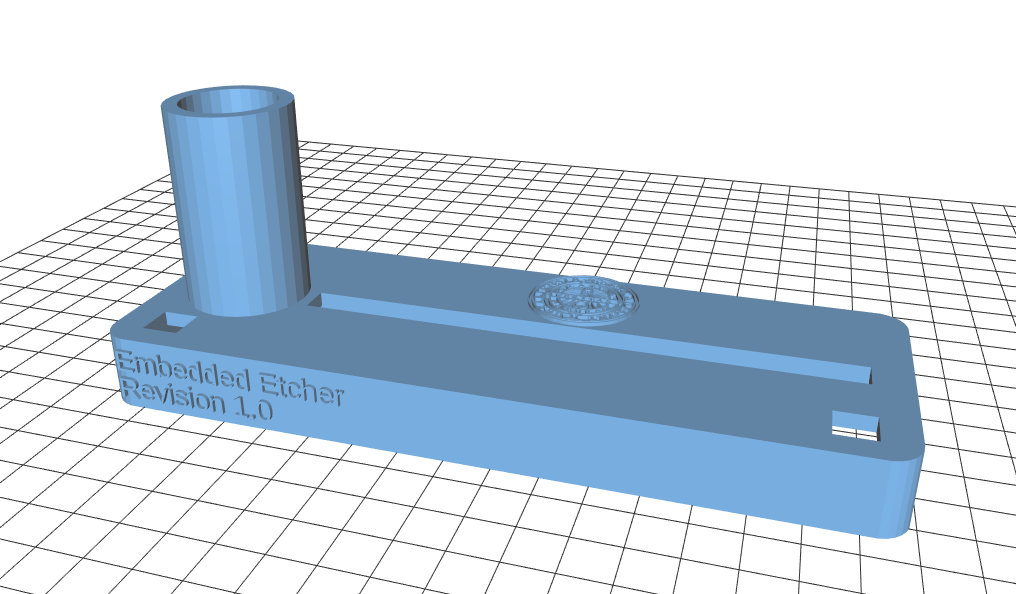
\includegraphics[width=0.6\textwidth]{./fig/lid}   
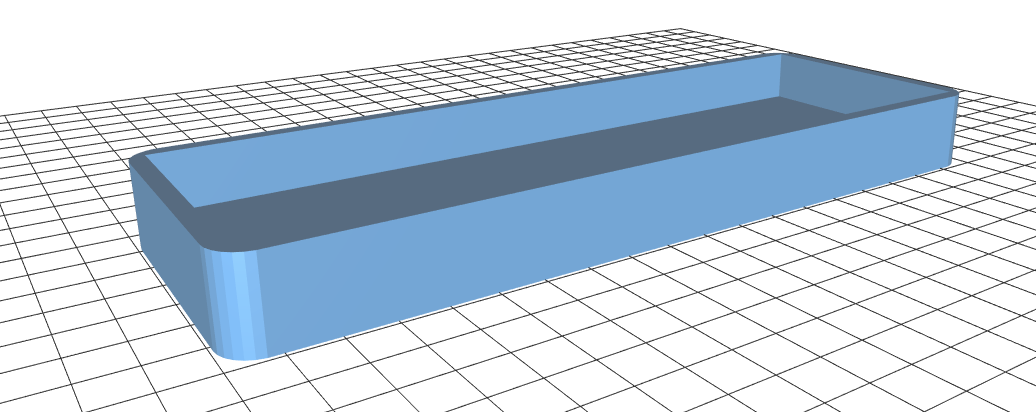
\includegraphics[width=0.6\textwidth]{./fig/floor} 
\caption[Lid and floor of the etching tank.]{Lid and floor of the etching tank.}   
\label{fig:lidFloor} 
\end{figure}

% \begin{figure}[H]
% \centering  
% 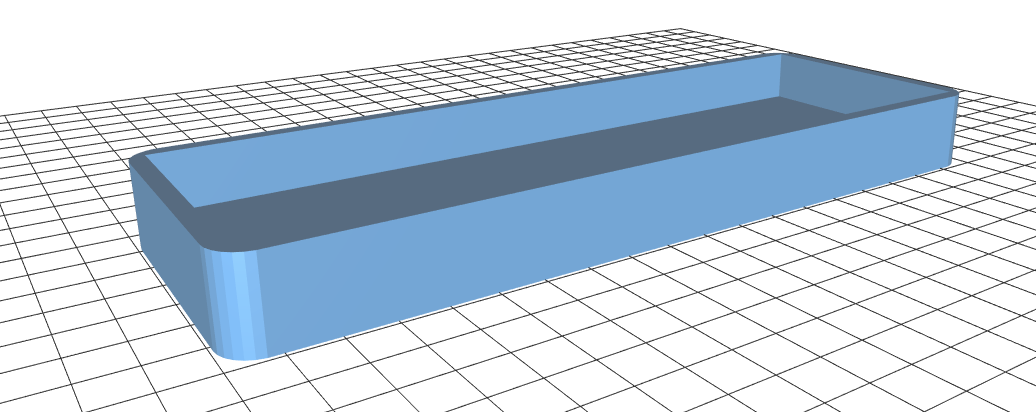
\includegraphics[width=0.6\textwidth]{./fig/floor}   
% \caption[Floor of the etching tank.]{Floor of the etching tank.}   
% \label{fig:floor} 
% \end{figure} 

\begin{figure}[H]
\centering  
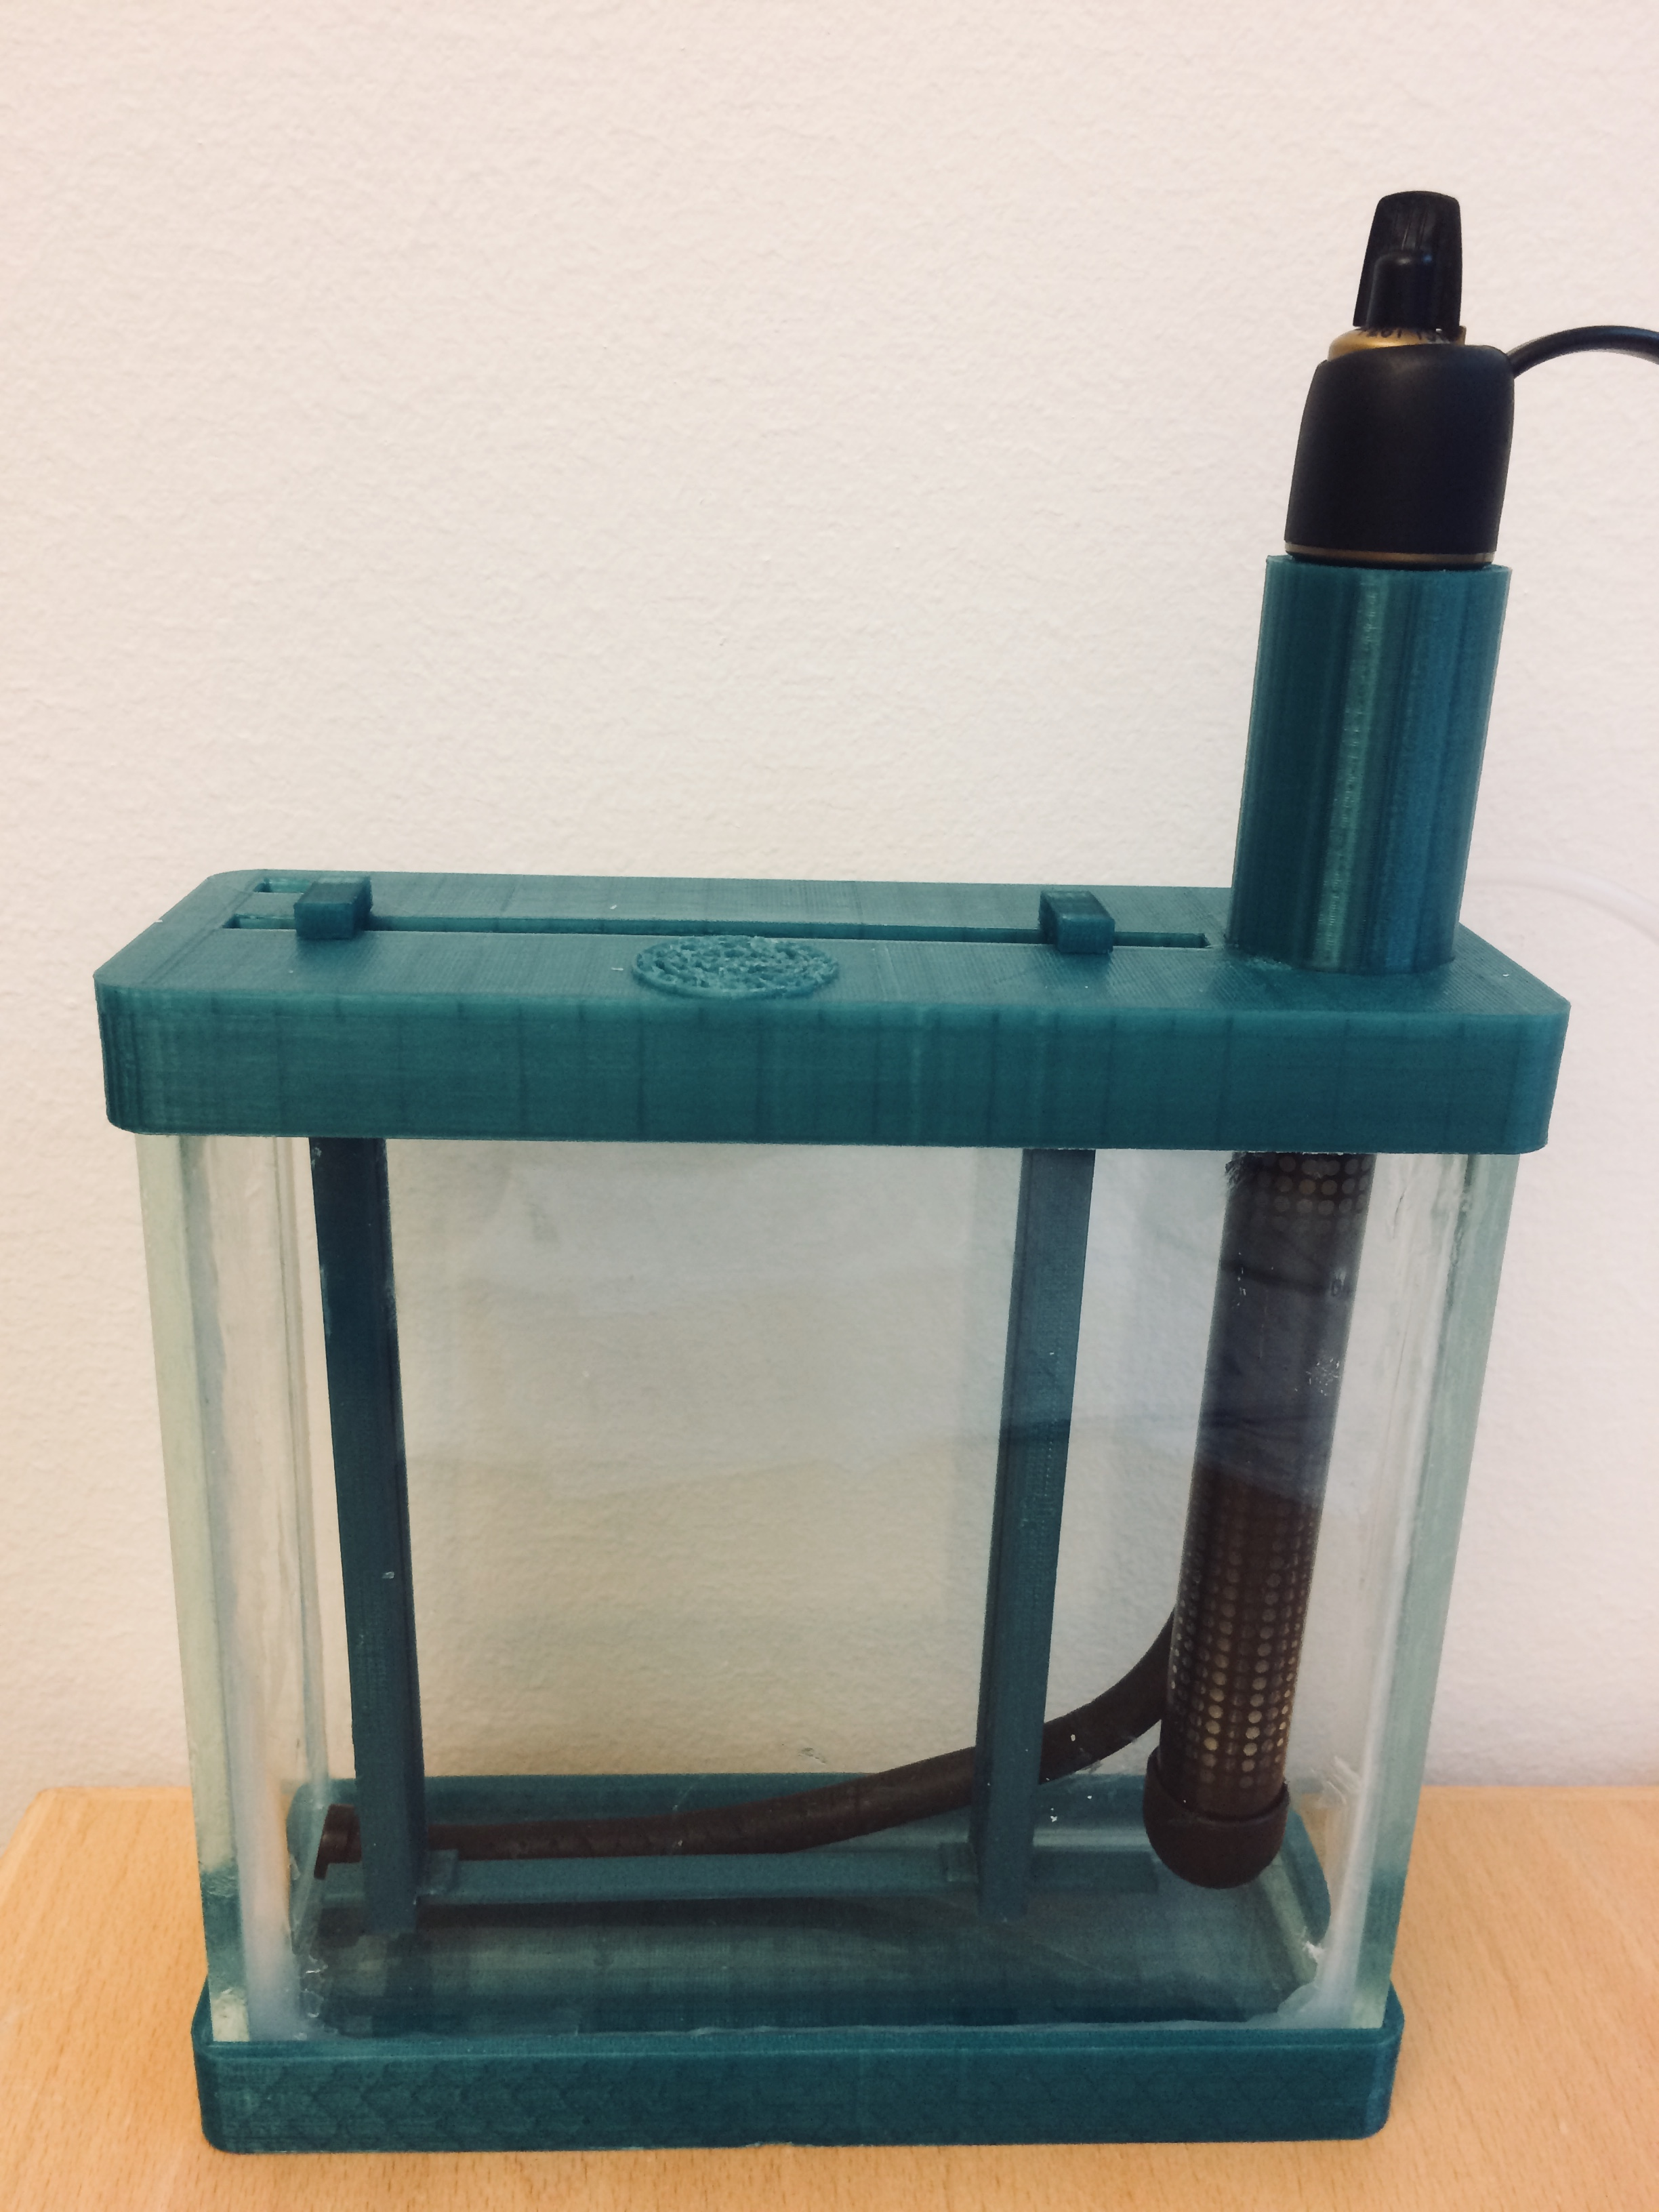
\includegraphics[width=0.6\textwidth]{./fig/tank}   
\caption[The etching tank.]{The etching tank.}   
\label{fig:tank} 
\end{figure}

\section{Operating System}
\label{sec:os}

\begin{figure}[H]                                                         
\centering          
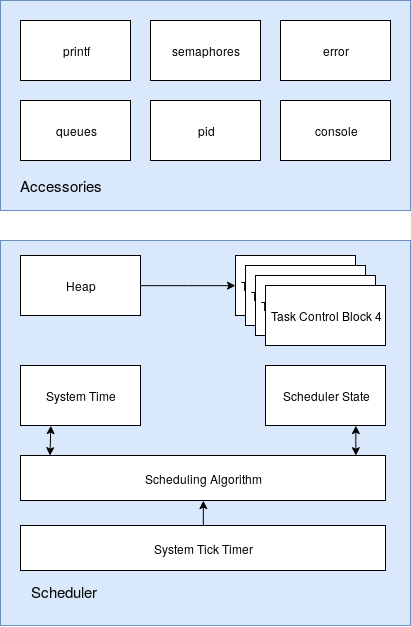
\includegraphics[width=0.5\textwidth]{./fig/redhead_os}   
\caption[Structure of the \gls{OS}]{Structure of the \gls{OS}}   
\label{fig:redhead_os}                                                       
\end{figure}  

In the course of the project a small real-time \gls{OS} has been developed. Fig. \ref{fig:redhead_os} shows how the \gls{OS} is structured. The operating system kernel consists out of a pretty simple scheduler, which is hooked up to the system tick timer, that the \myemph{Cortex-M3} (in the case of the \myemph{STM32F103RB}) provides. Configuring the system tick period is possible. With every system tick the scheduling algorithm is invoked. A state machine is deciding how to handle the system tick. Moreover, the scheduling is based on a binary heap, that contains pointers to the \glspl{TCB} of the tasks, which are supposed to be executed. A task control block is created, when a task is spawned by a programmer with. This works as follows:

\begin{minted}[baselinestretch=1, fontsize=\small, linenos,frame=single,framesep=5pt]{C}
/** Spawn a task.
 *
 * @param ifnc_ptr Pointer to the task function.
 * @param itask_name Internal task name.
 * @param iarguments Enables passing user-defined arguments to the task.
 * @param ipriority A higher value means a higher priority of the task.
 * @param oTaskHandle Pointer to TCB.
 * @retval 1 (task has been spawned) or 0 (FAILED)
 */
uint8_t osTaskCreate(void (*ifnc_ptr)(void*), char* itask_name, void* iarguments, 
	uint8_t ipriority, const osTCB_t* oTaskHandle);
\end{minted}

In general the \gls{OS} interface is frankly speaking inspired by FreeRTOS\texttrademark{}. One can also see, that the scheduling is priority based. The task with the highest priority is always executed as soon as the current task finished its job. Priorities can not be changed on run-time. Of course, as with any real-time \gls{OS} delay functions are available. \myemph{osTaskDelayUntil} is the more important one, as it allows periodic task execution. 

\begin{minted}[baselinestretch=1, fontsize=\small, linenos,frame=single,framesep=5pt]{C}
void task3(void* ptr)
{
	static uint32_t wakeup = 0;
	char* args = (char*)ptr;

	wakeup = osSchedulerGetSysT();
	DEBUG_MSG("%s here!\n\r", args);
	osTaskDelayUntil(wakeup, MS_2_TICKS(300));
}
\end{minted}

As shown in the example above the \gls{TCB} also holds a pointer to data, that can be passed to a task. 
\newpar 
Besides creating a easily understandable real-time \gls{OS} it was intended to provide some smooth infrastructure with it, or rather to equip it with some tools, so that one does not always have to reinvent the wheel, kicking off a new project. Therefore, the \gls{OS} comes with a growing set of accessories as for instance queues (cf. accessories in fig. \ref{fig:redhead_os}). 

\begin{minted}[baselinestretch=1, fontsize=\small, linenos,frame=single,framesep=5pt]{C}
void USART2_IRQHandler(void)
{
	/* USART2 receive buffer contains a char. */
	if(USART_GetITStatus(USART2, USART_IT_RXNE) == SET)
	{
		uint8_t data;
		data = USART_ReceiveData(USART2) & 0xFF;
		if(!osEnqueue(&usart_rx_q, (void*)&data))
			THROW_ERROR(E_USART_RX_BUFFER_OVERLOW);
	}

	/* USART2 transmit buffer empty. */
	if(USART_GetITStatus(USART2, USART_IT_TXE) == SET)
	{
		uint8_t data;
		if(osDequeue(&usart_tx_q, &data))
			USART_SendData(USART2, data);
		else
		{
			/* Nothing to send. Disable interrupt. */
			USART_ITConfig(USART2, USART_IT_TXE, DISABLE);
			tx_overflow = 0;
		}
	}
}
\end{minted}
The code example above shows how the error and the queue accessories can be used to implement the \gls{USART} \gls{IRQ} handler of the \myemph{STM32F103RB} elegantly. The \gls{USART} status register has to be checked for finding out which event triggered the interrupt. Either the transmit buffer is empty again and needs to be fed or the receive buffer contains a char, which needs to be stored somewhere. Both buffers are only as big as 8 bit, so one needs queues, that can be emptied and filled by concurrent processes. The \gls{OS} takes care of that. Also, in this example one can see how an error is passed to the according module in case, the receive buffer overflows. The idea is to have a proper log of what is going on in case the system fails (where did it go wrong and when). Also the sink for error logging can be changed (\gls{EEPROM} / \gls{USART} / screen).
\newpar 
Other accessories are 
\begin{itemize}
\item printf - A light version of \gls{GNU} printf. 
\item semaphores - Different kind of semaphores to get rid of data inconsistency problems that occur with concurrent processes e.g. tasks. 
\item pid - Infrastructure for \gls{PID} controll. 
\item console - A console to command the system and get feedback, similar to a terminal. 
\end{itemize}

The whole \myemph{Doxygen} documentation can be found on \myemph{Github}. 


% \section{Rotary encoder}
% The rotary encoder used for testing and development has a theoretically simple output, however it is of a rather bouncy and thus bad quality, as shown in figure~\ref{fig:re}. Depending on the turning direction either channel A or channel B gets low first and the first one gets high again while the second is still low.
% \begin{figure}[H]
% 	\centering
% 	\includegraphics[width=.8\linewidth]{./fig/re.jpg}
%     \label{fig:re}
% \end{figure}
% Due to many bounces, working with flags, similar to semaphores, is a good option to simply ignore all the bounces. However, one is then restricted to the frequency of calling \texttt{main()}.





%%%%%%%%%%%%%%%%%%%%%%%%%%%%%%%%%%%%%%%%%%%%%%%%%%%%%%%%%%%%%%%%%%%%%%%%%%%%%%%%%%%%%%
% Evaluation
%%%%%%%%%%%%%%%%%%%%%%%%%%%%%%%%%%%%%%%%%%%%%%%%%%%%%%%%%%%%%%%%%%%%%%%%%%%%%%%%%%%%%%

%%%%%%%%%%%%%%%%%%%%%%%%%%%%%%%%%%%%%%%%%%%%%%%%%%%%%%%%%%%%%%%%%%%%%%%%%%%%%%%%%%%%%%
%% Author:      Nils Weber and Maximilian Stiefel
%% Date:        23.12.2017
%% University:  Uppsala Universitet
%% Department:  Institutionen för informationsteknologi 
%% Course:      Embedded Control System Project
%% Project:     PRECISELY CONTROLLED DIY ETCHING MACHINE 
%%				FOR USAGE AT HOME AND IN SMALL LABS
%%%%%%%%%%%%%%%%%%%%%%%%%%%%%%%%%%%%%%%%%%%%%%%%%%%%%%%%%%%%%%%%%%%%%%%%%%%%%%%%%%%%%%

\chapter{Evaluation}
\label{chap:evaluation}
% Describe the status of the work. What has been achieved?
The whole project is a strict work in progress, which is not finished yet. Different components have a different maturity. 
\newpar 
Tab. \ref{tab:os_status_quo} reflects the status quo of the \gls{OS}. It can certainly not keep up with modern \glspl{OS}. Nevertheless, it is easily comprehensible, because of its small footprint, and provides a bit another approach as a pure solution for real-time \glspl{OS} for embedded applications with useful accessories in this field.  

\begin{table}[H]
\centering
\begin{tabularx}{\textwidth}{lcX}
\textbf{Component} & \textbf{Working} & \textbf{Problem} \\\hline
Non-preemptive Scheduling & \checkmark	& Round-robin scheduling is not guaranteed among tasks having the same priority. \\
Preemptive Scheduling & \checkmark	& \\	
System Tick Configuration & \checkmark	& \\
Error Logging & \checkmark	& Only supports one sink (\gls{USART}) so far. \\
printf & \checkmark	& Only supports the options \%d, \%f, \%c and \%s currently. \\
Queues & \checkmark	& Only supports one kind of queue, which is useful for a producer-consumer scenarios. \\
Semaphores & & \\
\gls{PID} controller infrastructure & & \\
Console & & \\
\hline
\end{tabularx}
\caption{Status Quo \gls{OS}}
\label{tab:os_status_quo}
\end{table}

The \gls{UV} light hardware has been simulated with the help of \myemph{LTSpice} quite extensively. After gaining support from Yi Wang and convincing the department to pay these companies for their products and services respectively, both \glspl{PCB} introduced earlier have been manufactured in China by the company \myemph{Elecrow} (\hyperref{http://www.elecrow.com}{Elecrow}). Also, the components have been ordered in the USA from the distributor \myemph{Digikey} and are available. The boards have not yet been assembled and tested. The planned intend to get rid of mercury, mentioned in chapter \ref{chap:background}, has been pursued consequently. It is an absolutely revolutionary feature, that this \gls{UV} exposure unit does not use fluorescent lamps like the most common type the competitors offer on the market right now. A housing has been built from wood, which is cheaper and rather environmentally friendly. The current mechanics allow single-sided \gls{UV} light exposure.  

\begin{table}[H]
\centering
\begin{tabularx}{\textwidth}{lcX}
\textbf{Component} & \textbf{Working} & \textbf{Problem} \\\hline
No mercury & \checkmark & \\
Double-sided UV light exposure & & \\
Precisely controlled light intensity & \checkmark & \\
Digital and elegant user interface & \checkmark & \\
Hardware design ready & \checkmark & \\
Hardware assembled and tested & & \\
No expensive metal housings & \checkmark & \\
\gls{DAC} driver & & \\
\gls{OLED} driver & & \\
Rotary encoder driver & & \\
\hline
\end{tabularx}
\caption{Status Quo \gls{UV} light}
\label{tab:os_status_quo}
\end{table}


The etching bath temperature control is in an earlier stage of development, where success was for a long time hindered by a driver issue with the \gls{ADC} on a similar STM32-chip. For development the STM32L073RZ was used, for the simple reason of immediate availability. However, the \gls{ADC} on this specific chip has had problems reading the values properly until now. Without actual data from the temperature sensor the rest of the system could only be implemented but not tested. A simple on-off controller has been tested successfully, the implementation with proportional and inertia correction has not yet been tested successfully.



\begin{table}[H]
\centering
\begin{tabularx}{\textwidth}{lcX}
\textbf{Component} & \textbf{Working} & \textbf{Problem} \\\hline
Digital and elegant user interface & \checkmark & \\
Hardware design ready & & \\
Hardware assembled and tested & & Heater needs to be "hacked" for control \\
Additive manufactured housing & \checkmark & PCB holder needs improvement \\
\gls{ADC} driver for NTC & \checkmark & \\
\gls{I2C} driver & \checkmark & \\
\gls{OLED} driver & \checkmark & \\
Rotary encoder driver & \checkmark & Low-pass filter missing \\
On-off controller & \checkmark & \\
On-off controller with corrections & & \\
\hline
\end{tabularx}
\caption{Status Quo etching bath}
\label{tab:etching_status_quo}
\end{table}

%%%%%%%%%%%%%%%%%%%%%%%%%%%%%%%%%%%%%%%%%%%%%%%%%%%%%%%%%%%%%%%%%%%%%%%%%%%%%%%%%%%%%%
% Conclusion
%%%%%%%%%%%%%%%%%%%%%%%%%%%%%%%%%%%%%%%%%%%%%%%%%%%%%%%%%%%%%%%%%%%%%%%%%%%%%%%%%%%%%%

%%%%%%%%%%%%%%%%%%%%%%%%%%%%%%%%%%%%%%%%%%%%%%%%%%%%%%%%%%%%%%%%%%%%%%%%%%%%%%%%%%%%%%
%% Author:      Nils Weber and Maximilian Stiefel
%% Date:        23.12.2017
%% University:  Uppsala Universitet
%% Department:  Institutionen för informationsteknologi 
%% Course:      Embedded Control System Project
%% Project:     PRECISELY CONTROLLED DIY ETCHING MACHINE 
%%				FOR USAGE AT HOME AND IN SMALL LABS
%%%%%%%%%%%%%%%%%%%%%%%%%%%%%%%%%%%%%%%%%%%%%%%%%%%%%%%%%%%%%%%%%%%%%%%%%%%%%%%%%%%%%%

\chapter{Conclusion and Future Work}
\label{chap:conclusion}
% Summarize and conclude. Give a brief outlook as well on what will be done in future. 

The \gls{OS} kernel works and the system is ready to be deployed. A couple of accessories as are not implemented at all yet. Others need to be upgraded. The kernel is also subject to improvements. It shall be possible for the programmer to chose whether the scheduling is preemptive or non-preemptive. Also, it shall be possible to assign a stack size to a task and make sure it is not overflowed. 
\newpar 
The \gls{UV} light development put forth a complex four layer extension board for the \myemph{Nucleo-F103RB} from \myemph{STM}, including a sophisticated \gls{LED} driver using a linear regulator approach. The circuits on the board have been laid out, simulated and in a next step they will be tested. Moreover, a mechanical design has been sketched and built up. Unfortunately, it only supports single-sided \gls{UV} light exposure and causes a lot of manual work building it, which is something to be solved in the near future. One idea is to use some \gls{FDM} parts combined with two \glspl{PCB}, 128 \glspl{LED} each, to make double-sided exposure and an easy assembly possible. Most of the driver software implementation still has to be done and the whole system has to be integrated. 
\newpar
The temperature control development for the etching bath is ready for testing as soon as the temperature sensor is read correctly from the \gls{ADC}. These tests will show if the implemented improved on-off control will deliver sufficient results or if the heater has to be controlled with a constant current controller. When that is decided further steps regarding hardware design can be made.
Also, the current implementation has to be ported to the \gls{OS}, which should not entail much work, as it is structured in a fitting way already. 

%%%%%%%%%%%%%%%%%%%%%%%%%%%%%%%%%%%%%%%%%%%%%%%%%%%%%%%%%%%%%%%%%%%%%%%%%%%%%%%%%%%%%%
% Bibliography and Appendix
%%%%%%%%%%%%%%%%%%%%%%%%%%%%%%%%%%%%%%%%%%%%%%%%%%%%%%%%%%%%%%%%%%%%%%%%%%%%%%%%%%%%%%

\clearpage
\pagenumbering{Roman}
\setcounter{page}{\value{roman}}
\pagestyle{empty}

\printbibliography[heading=bibintoc]

%%%%%%%%%%%%%%%%%%%%%%%%%%%%%%%%%%%%%%%%%%%%%%%%%%%%%%%%%%%%%%%%%%%%%%%%%%%%%%%%%%%%%%
% Appendix
%%%%%%%%%%%%%%%%%%%%%%%%%%%%%%%%%%%%%%%%%%%%%%%%%%%%%%%%%%%%%%%%%%%%%%%%%%%%%%%%%%%%%%
\appendix
% Introduce new geometry to be able to have more space for appendix
\newgeometry{lmargin={2.5cm},rmargin={2.5cm},tmargin={0cm},bmargin={1,5cm}}
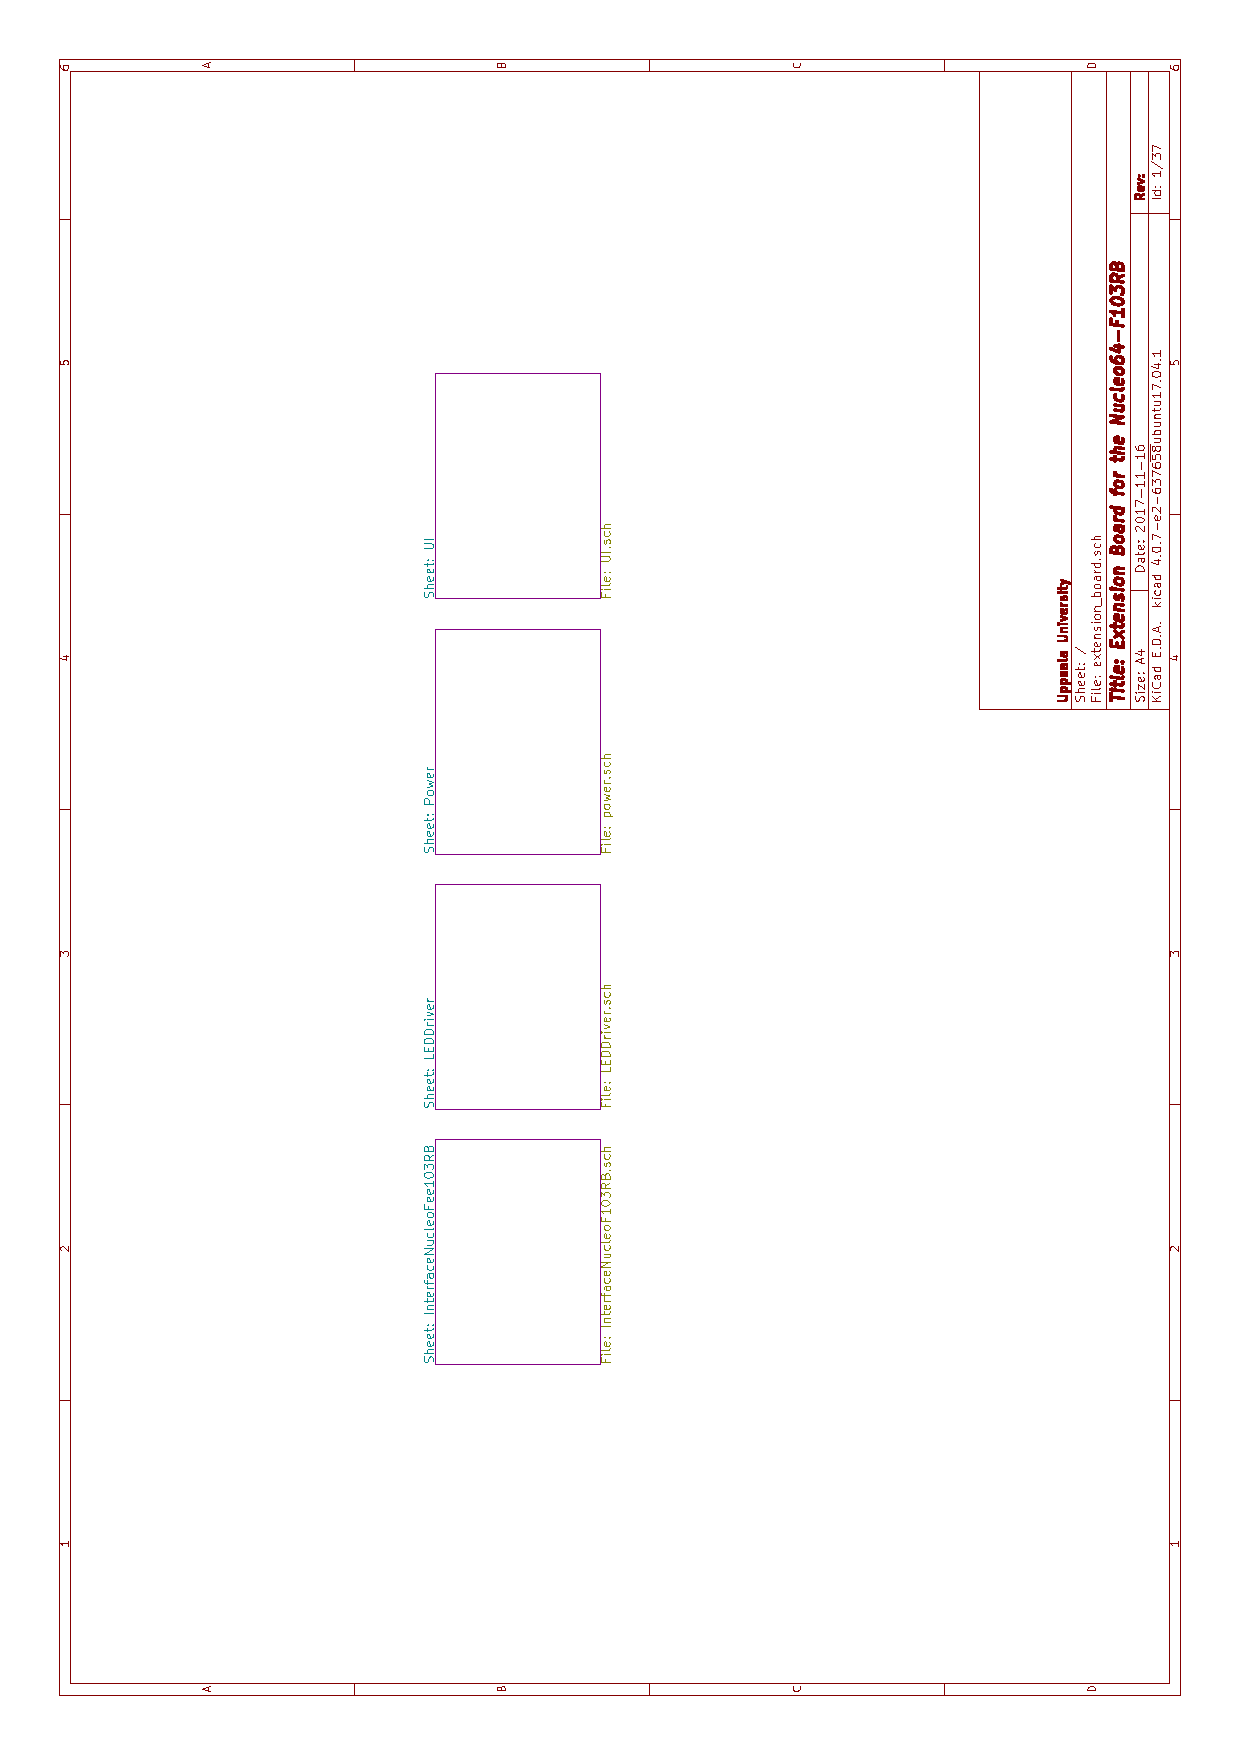
\includepdf[pages={1},scale=0.8,pagecommand=\chapter{Schematics Extension Board}\label{append:extension}]{./fig/schematics_extension_board.pdf}
\includepdf[pages={2-3, 35-37},scale=0.8,pagecommand={}]{./fig/schematics_extension_board.pdf}

\chapter{Technical drawings of PCB-holder}
\label{append:techDrawPCB}

\begin{figure}[H]
\centering  
\includegraphics[width=0.8\textwidth]{./fig/pcb_holder_crossbar}
\caption{Technical Drawing: Crossbar} 
\end{figure} 

\begin{figure}[H]
\centering  
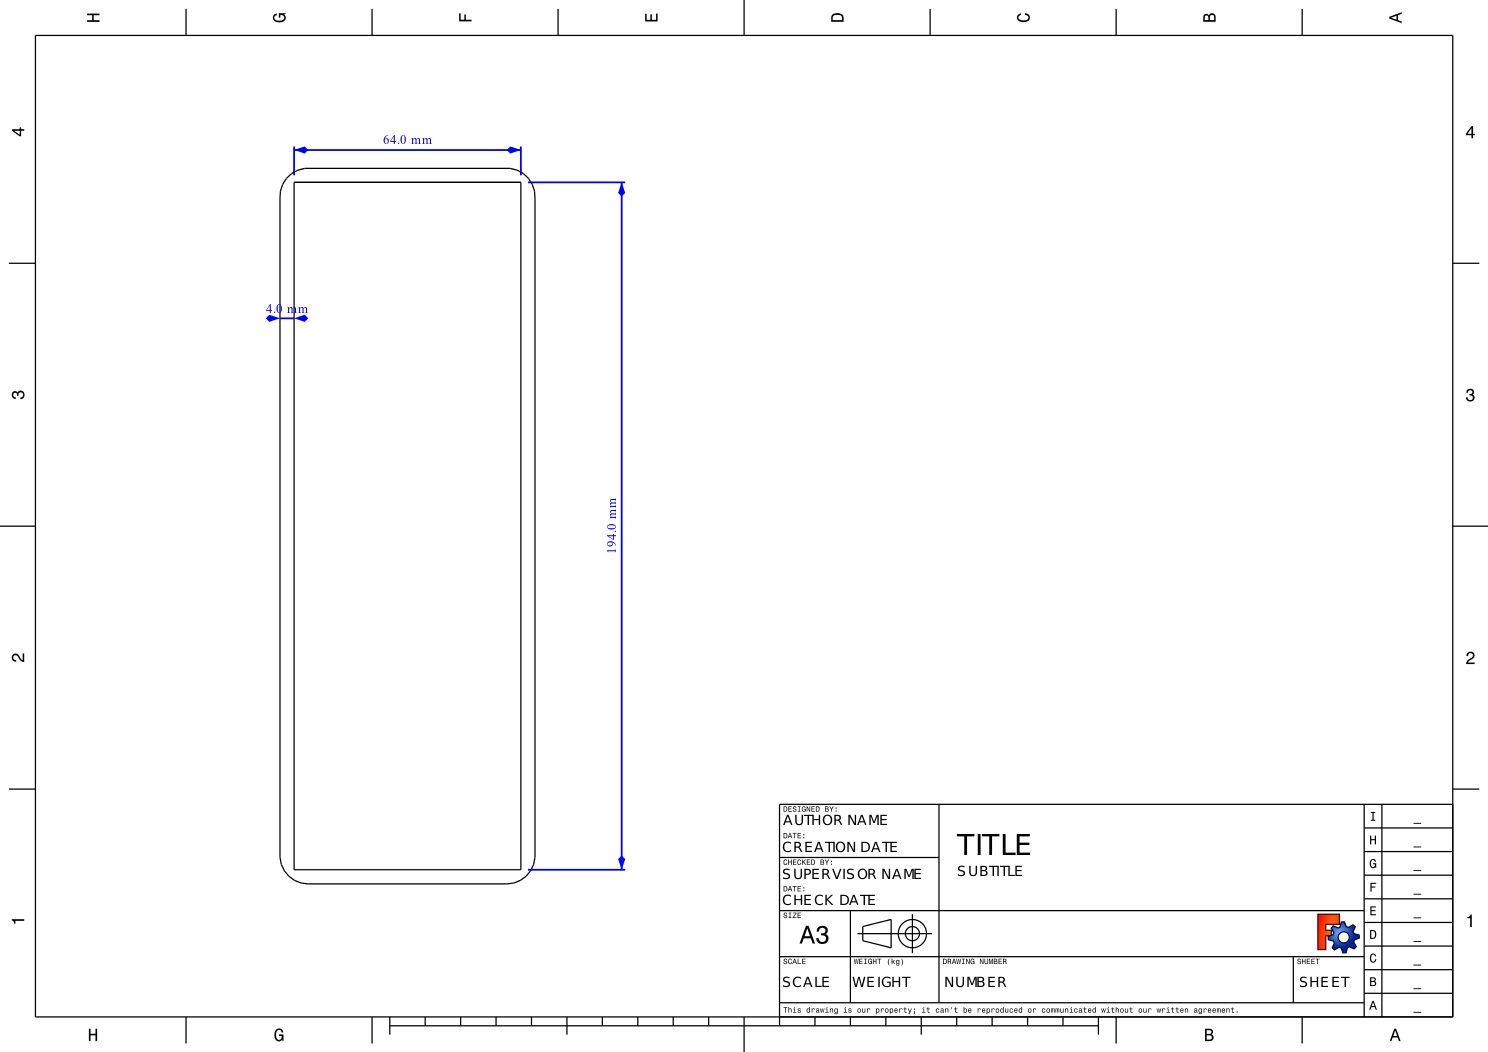
\includegraphics[width=0.8\textwidth]{./fig/pcb_holder_floor_prot}   
\caption{Technical Drawing: Floor}
\end{figure} 

\newgeometry{lmargin={2.5cm},rmargin={2.5cm},tmargin={2.5cm},bmargin={2.5cm}}

\begin{figure}[H]
\centering  
\includegraphics[width=0.8\textwidth]{./fig/pcb_holder_holder}   
\caption{Technical Drawing: Holder}
\end{figure} 

\begin{figure}[H]
\centering  
\includegraphics[width=0.8\textwidth]{./fig/pcb_holder_lid}  
\caption{Technical Drawing: Lid} 
\end{figure} 

\end{document}
